%****************************************************
%	CHAPTER 3 - Dynamics
%****************************************************
\chapter{Kinematics \& Dynamics}
\label{ch:dynamics}
%====================================================
The following generally applicable, rigid body dynamics are first derived with respect to net forces and torques. Thereafter, those dynamics are adapted to the non-linear, multibody case where constrained relative rotational motion between bodies is permitted. Following that, aerodynamic effects are incorporated into the plant's model. Finally a consolidated, quaternion based plant model is presented which is used for the later control plant development in Ch:\ref{ch:control}.
%====================================================
\section{Rigid Body Dynamics}
\label{sec:dynamics.rigidbody}
%====================================================
\subsection{Lagrange Derivation}
\label{subsec:dynamics.rigidbody.lagrange}
%====================================================
Fundamentally any body, rigid or otherwise, can undergo two kinds of motion, namely rotational and translation. Often a Lagrangian approach for combined angular and translational movements is used to derive the differential equations of motion for each degree of freedom \cite{classicaldynamics,rotationrigidbody}. The Lagrangian principle ensures that (translational and rotational) kinematic energies and potential energy are conserved throughout the system's trajectory progression. When combined with Euler-Rotational equations, the Euler-Lagrangian\cite{lagrange-formalism} formulation fully defines the aerospace 6-DOF equation set.
\par
Lagrangian formalism is regarded as especially useful in non-Cartesian (\emph{spherical etc\ldots}) co-ordinate frames or multi-body systems. With that being said, Cartesian co-ordinates were defined in Sec:\ref{subsec:proto.conventions.motoraxis} for this system. An alternative relative co-ordinate system could be used for implicit-Euler based dynamics \cite{autonomousrobotseuler}.
Rigid body dynamics in a Cartesian co-ordinate frame do lend themselves to Newtonian mechanics. The Newton-Euler and Euler-Lagrange formulations both result in the same differential equations of motion, but follow different derivations. The Lagrangian operator, $\mathcal{L}$, is a term consisting of the difference between kinetic and potential energies, $T$ and $U$ respectively. Considering some generalized path co-ordinates $\vec{\mathbf{r}}(t)$, for both position $\vec{\xi}$ and attitude $\vec{H}$ co-ordinates;
\begin{equation}\label{eq:generalpath}
\vec{\mathbf{r}}(t)=\begin{bmatrix}
\vec{\xi} & \vec{H}
\end{bmatrix}^T~~~~\in\mathcal{F}^{\Lambda}
\end{equation}
The co-ordinates in Eq:\ref{eq:generalpath} are generalized and taken with respect to some shared frame $\Lambda$. Those generalized co-ordinates are later refined to Cartesian body co-ordinates with respect to the inertial frame. The Lagrangian is, by definition:
\begin{subequations}
\begin{equation}\label{eq:lagrangian.a}
\mathcal{L}(\vec{\mathbf{r}},\dot{\vec{\mathbf{r}}},t)=T(\vec{\mathbf{r}},\dot{\vec{\mathbf{r}}})-U(\vec{\mathbf{r}},\dot{\vec{\mathbf{r}}})
\end{equation}
With the trajectory's kinetic and potential energy function(s) are $T$ and $U$ respectively. Introducing a rigid body's general (translational and rotational) kinetic and potential energies, together in the shared reference frame $\mathcal{F}^\Lambda$. 
\newpage
There is no angular contribution of potential stored energy, so $U(\vec{\mathbf{r}},\dot{\vec{\mathbf{r}}})$ depends only only gravitational potential energy. With gravity is defined as $G_I=\begin{bmatrix} 0&0&-9.81 \end{bmatrix}^T~[\text{m.s}^{-2}]$~in the Inertial frame,$\in\mathcal{F}^I$, the Lagrangian scalar is then:
\begin{equation}\label{eq:lagrangian.b}
\mathcal{L}(\vec{\mathbf{r}},\dot{\vec{\mathbf{r}}},t)=\frac{1}{2}\dot{\vec{\xi}}^{~T}(m_b)\dot{\vec{\xi}}+\frac{1}{2}\dot{\vec{H}}^{~T}(J_b)\dot{\vec{H}}-m\vec{G}_{\Lambda}z
\end{equation}
\end{subequations}
Noting that $J_b$ is body's inertial matrix aligned and translated with respect to the common frame $\mathcal{F}^{\Lambda}$. The Euler-Lagrange formulation equates partial derivatives of the Lagrangian to any generalized forces, $\vec{\mathbf{V}}$, acting on the system in $\Lambda$. In the rigid body motion case the generalized forces are net forces $\vec{F}_{net}$ torques $\vec{\tau}_{net}$ in the shared frame $\in\mathcal{F}^{\Lambda}$.
\begin{equation}\label{eq:euler-lagrange}
\frac{d}{dt}\bigg(\frac{\delta \mathcal{L}}{\delta \dot{\vec{\mathbf{r}}}}\bigg)-\frac{\delta \mathcal{L}}{\delta \vec{\mathbf{r}}} = \vec{\mathbf{V}} = \begin{bmatrix}
\vec{F}_{net}\\
\vec{\tau}_{net}
\end{bmatrix}~~~~\in\mathcal{F}^{\Lambda}
\end{equation}
Then taking the partial derivatives of Eq:\ref{eq:lagrangian.b} with respect to the path co-ordinates $\vec{\mathbf{r}}(t)$:
\begin{subequations}
\begin{equation}\label{eq:partial.a}
\frac{\delta \mathcal{L}}{\delta \vec{\mathbf{r}}}=\begin{bmatrix}
m_b\vec{G}_\Lambda\\
0
\end{bmatrix}~~~~\in\mathcal{F}^{\Lambda}
\end{equation}
\vspace{-5pt}
\begin{equation}\label{eq:partial.b}
\frac{d}{dt}\bigg(\frac{\delta \mathcal{L}}{\delta \dot{\vec{\mathbf{r}}}}\bigg)=\bigg[
\frac{d}{dt}m_b\dot{\vec{\xi}} ~~~ \frac{d}{dt}J_b\dot{\vec{H}}\bigg]^T~~~~\in\mathcal{F}^{\Lambda}
\end{equation}
\end{subequations}
Where $\vec{G}_\Lambda$ is the gravitation force in the common frame $\mathcal{F}^\Lambda$ which $\mathcal{L}(\vec{\mathbf{r}},\dot{\vec{\mathbf{r}}})$ is with respect to. The body mass $m_b$ and inertia $J_b$ could potentially have some non-zero time derivative, but here are considered to be constant. Time varying inertias are addressed later in Sec:\ref{subsec:dynamics.nonlinearities.gyrotorques}. Any vector in a rotating generalized coordinate system has time derivative relative to another reference frame as per the Reynolds Transportation Theorem\cite{reynolds}:
\begin{equation}\label{eq:reynolds}
\frac{d\vec{f}}{dt_a}=\frac{d\vec{f}}{dt_b}+\vec{\omega}_{a/b}\times\vec{f}
\end{equation}
So applying Eq:\ref{eq:reynolds} to the partial derivatives in Eq:\ref{eq:partial.b} and further defining the generalized co-ordinates $[\vec{\xi},~\vec{H}]^T$ as 6-DOF Cartesian body coordinates with respect to an inertial frame (the body frame $\mathcal{F}^b$ and inertial frame $\mathcal{F}^I$). Reiterating that the angular orientations $\vec{\xi}$ are with respect to a common frame $\mathcal{F}^{\Lambda}$, unlike Euler angles $\vec{\eta}\in\mathcal{F}^{v2,v1,I}$. Recalling the definition of attitude in a common frame $\vec{\eta}_b$ from Eq:\ref{eq:angular-rates.b}, where $\vec{\omega}_b=\dot{\vec{\eta}}_b$ and $\vec{\eta}_b\in\mathcal{F}^{b}$, the trajectory is refined: 
\begin{equation}
\vec{\mathbf{r}}=\begin{bmatrix}
\vec{\xi}&
\vec{H}
\end{bmatrix}^T
\triangleq
\begin{bmatrix}
\vec{\mathcal{E}}_{\hspace{3pt}}\\
\vec{\eta}_{b}
\end{bmatrix}
\rightarrow
\dot{\vec{\mathbf{r}}}=
\begin{bmatrix}
\dot{\vec{\xi}} & \dot{\vec{H}}
\end{bmatrix}^T
\triangleq
\frac{d}{dt}
\begin{bmatrix}
{\vec{\mathcal{E}}}_{\hspace{3pt}}\\
\vec{\eta}_b
\end{bmatrix}
=
\begin{bmatrix}
\vec{\nu}\\
\vec{\omega}
\end{bmatrix}~~~~
\in \mathcal{F}^b
\end{equation}
It then follows that the Lagrangian in Eq:\ref{eq:lagrangian.b} changes to:
\begin{subequations}
\begin{equation}\label{eq:3.7a}
\mathcal{L}=\frac{1}{2}\vec{\nu}^{~T}(m_b)\vec{\nu} + \frac{1}{2}\vec{\omega}^{~T}(J_b)\vec{\omega}
-m_b\vec{G}_b z~~~~\in\mathcal{F}^b
\end{equation}
\vspace{-10pt}
\begin{equation}
\frac{d}{dt}\bigg(\frac{\delta \mathcal{L}}{\delta \dot{\vec{\mathbf{r}}}}\bigg)=\bigg[
m_b\frac{d}{dt}\vec{\nu} ~~~ J_b\frac{d}{dt}\vec{\omega}\bigg]^T
\end{equation}
\vspace{-5pt}
\begin{equation}
\rightarrow m_b\frac{d}{dt}\vec{\nu}=m_b\dot{\vec{\nu}}+\vec{\omega}_{I/b}\times\vec{\nu}
\end{equation}
\vspace{-5pt}
\begin{equation}
\rightarrow J_b \frac{d}{dt}\vec{\omega}=J_b\dot{\vec{\omega}}+\vec{\omega}_{I/b}\times J_b\vec{\omega}
\end{equation}
\end{subequations}
Which, when substituted back into the Euler-Lagrange formulation Eq:\ref{eq:euler-lagrange}, produces the familiar Newton-Euler rigid body equations for translational and rotational motion;
\begin{subequations}\label{eq:newton}
\begin{equation}\label{eq:newton.a}
\vec{F}_{net}=m_b\dot{\vec{\nu}}+\vec{\omega}_b\times m_b \vec{\nu} - m_bR_I^b(-\eta) \vec{G}_I~~~~\in\mathcal{F}^b
\end{equation}
\vspace{-15pt}
\begin{equation}\label{eq:newton.b}
\vec{\tau}_{net}=J_b\dot{\vec{\omega}}_b+\vec{\omega}_b\times J_b\vec{\omega}_b~~~~\in\mathcal{F}^b
\end{equation}
\end{subequations}
Reiterating that $\vec{\eta}_b\not=\vec{\eta}$ because each Euler Angle is defined in a sequentially rotated reference frame. Four equations then completely describe a body position's and attitude's state dynamics:
\begin{subequations}\label{eq:states}
\begin{equation}\label{eq:states.a}
\dot{\vec{\mathcal{E}}}=R_b^I(-\eta)\vec{\nu}~~~~\in\mathcal{F}^I
\end{equation}
\vspace{-14pt}
\begin{equation}\label{eq:states.b}
\vec{F}_{net}=m_b\dot{\vec{\nu}}+\vec{\omega}_b\times m_b\vec{\nu} -m_b R_I^b(-\eta)\vec{G}_I ~~~~\in\mathcal{F}^b
\end{equation}
\vspace{-12pt}
\begin{equation}\label{eq:states.c}
\dot{\vec{\eta}}=\Phi(\eta)\vec{\omega}_b~~~~\in\mathcal{F}^{v2,v1,I}
\end{equation}
\vspace{-12pt}
\begin{equation}\label{eq:states.d}
\vec{\tau}_{net}=J_b\dot{\vec{\omega}}_b+\vec{\omega}_b\times J_b\vec{\omega}_b~~~~\in\mathcal{F}^b
\end{equation}
\end{subequations}
Where $\Psi(\eta)$ is the Euler matrix defined previously in Eq:\ref{eq:angular-rates.c}. State differentials from Eq:\ref{eq:states} can be simplified to a set of two equations defined in the reference frames of the state variables which they represent. The non-linear form of those equations substitutes $d\vec{\eta}/dt=\Phi(\eta)\vec{\omega}_b$ into the Lagrangian derivative, Eq:\ref{eq:partial.b}.
\begin{equation}
\frac{d}{dt}\bigg(\frac{\delta \mathcal{L}}{\delta \dot{\mathbf{r}}}\bigg)=\bigg[m_b\frac{d}{dt}\vec{\nu}~~~J_b\frac{d}{dt}\dot{\vec{\eta}}_b\bigg]^T\Rightarrow\bigg[m_b\frac{d}{dt}\vec{\nu}~~~J_b\frac{d}{dt}\Phi(\eta)\vec{\omega}_b\bigg]^T
\end{equation}
This only affects the angular component as the two kinetic energies are independent of one another. Applying the differential chain rule yields:
\begin{equation}
J_b\frac{d}{dt}\Phi(\eta)\vec{\omega}_b=J_b\big(\Phi\dot{(\eta)}\vec{\omega}_b+\Phi(\eta)\dot{\vec{\omega}}_b \big)
\end{equation}
Drawing from \cite{autonomousrobotseuler} and recognizing that $J_b$ must be transformed to the common intermediate Euler axes, $\mathbb{J}=\Psi(\eta)^TJ_b\Psi(\eta)$. The state differential equation for angular acceleration in Eq:\ref{eq:newton.b}, then defined in intermediate (non-inertial) Euler frames for each angle, becomes:
\begin{subequations}\label{eq:nonlinear}
\begin{equation}\label{eq:nonlinear.a}
M(\eta)\ddot{\vec{\eta}}+C(\eta,\dot{\eta})\dot{\vec{\eta}}=\Psi(\eta)\vec{\tau}_{net}~~~~\in\mathcal{F}^{v2,v1,I}
\end{equation}
\vspace{-15pt}
\begin{equation}\label{eq:nonlinear.b}
M(\eta)=\Psi(\eta)^TJ_b\Psi(\eta)
\end{equation}
\vspace{-10pt}
\begin{equation}\label{eq:nonlinear.c}
C(\eta,\dot{\eta})=-\Psi(\eta)J_b\Psi\dot{(\eta)}+\Psi(\eta)^T \big[\Psi(\eta)\dot{\vec{\eta}}\big]_{\times}J_b\Psi(\eta)
\end{equation}
\end{subequations}
The relationship $\dot{\Phi}=\Phi\dot{\Psi}\Phi$ was used to simplify Eq:\ref{eq:nonlinear}, the singularity in $\Phi$ still remains. The equation in Eq:\ref{eq:nonlinear.a} fully describes the state derivative $\ddot{\vec{\eta}}$ in its own reference frame(s), $\mathcal{F}^{v2,v1,I}$. The two differential equations which fully describe the entire body's motion are then:
\begin{subequations}\label{eq:rigid-frame}
\begin{equation}\label{eq:rigid-frame.a}
\vec{F}_{net}=m_b\dot{\vec{\mathcal{E}}}+R_b^I(-\eta)\vec{\omega}_b \times m_b \dot{\vec{\mathcal{E}}}-m_b\vec{G}_I~~~~\in\mathcal{F}^I
\end{equation}
\vspace{-10pt}
\begin{equation}\label{eq:rigid-frame.b}
\vec{\tau}_{net}=\Psi(\eta)^{-1}M(\eta)\ddot{\vec{\eta}}+\Psi(\eta)^{-1}C(\eta,\dot{\eta})~~~~\in\mathcal{F}^{v2,v1,I}
\end{equation}
\end{subequations}
\par
The generalized net forces and torques acting on the body, $\vec{F}_\mu$ and $\vec{\tau}_\mu$ respectively, are the system's controllable inputs which are directly affected by the system's actuators. How the actuator suite affects the net forces and torques depend on the actuator's associated effectiveness function. In the general case, which is refined in Sec:\ref{sec:dynamics.aero}, the control inputs for a quadrotor are typically as follows. The net force acting on the system is simply the sum of all thrust forces produced by rotating propellers $\vec{T}(\Omega_i)$;
\begin{subequations}
\begin{equation}
\vec{F}_\mu = \sum_{i=1}^4 \vec{T}(\Omega_i)~~~~[\text{N}],~\in\mathcal{F}^b
\end{equation}
Similarly the net torque is the sum of all \emph{differential} torque arms produced from opposing propeller thrust vectors.
\begin{equation}
\vec{\tau}_\mu = \sum_{i=1}^4 \vec{l}_i \times \vec{T}(\Omega_i)~~~~[\text{N.m}],~\in\mathcal{F}^{b}
\end{equation}
\end{subequations}
Where $\vec{T}(\Omega_i)$ is the $i^{th}$ motor's thrust vector, fixed in the $\hat{Z}_b$ direction. The thrust vectors could potentially be $\in\mathbb{R}^3$. Similarly $\vec{l}_i$ is that thrust vector's perpendicular displacement from the origin $\mathbf{O}_b$. The above equations are still applicable to any 6 DOF body, common simplifications applied to the system(s) for quadrotor control are explored in App:\ref{app:equations.standard}. Aspects unique to (multibody) aerospace frames are now introduced. Obviously the contextual focus is on quadrotor and tilting quadrotor platforms\ldots
%====================================================
\subsection{Rotation Matrix Singularity}\label{subsec:dynamics.rigidbody.singularity}
%====================================================
The singularity inherent to Euler Angle parametrization is often mentioned but far less common is the mathematical demonstration of how that singularity manifests itself.  A singularity occurs for some matrix $A$ in $\vec{y}=A\vec{x}$ has a zero determinate, losing rank and differentiability. The combined rotation matrix from the $\mathcal{F}^{I}$ to $\mathcal{F}^{b}$ is the singular component of an Euler parametrized sequence. Considering the case of a rotational 3-axis gimbal system(Fig:\ref{fig:gimbal}) which mimics the sequential nature of the Euler set. When the intermediary sequenced rotational angle is at $\pi/2$, the remaining two axes become co-linear (Fig:\ref{fig:gimbal-lock}). In Z-Y-X rotation sequence adopted in this work, the singularity occurs from the rolling angle $\theta$ about $\hat{Y}$. Both the pitch $\phi$ or yaw $\psi$ rotations will subsequently have the same rotational effect. Such a situation results in as a loss of a degree of freedom.
\begin{figure}[htbp]
\begin{subfigure}{0.5\textwidth}
\centering
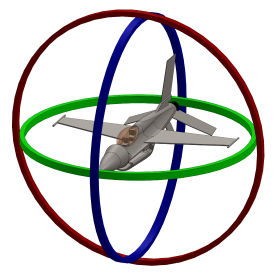
\includegraphics[width=0.9\textwidth]{figs/gimbal}
\caption{3-Axis gimbal}
\label{fig:gimbal}
\end{subfigure}
\begin{subfigure}{0.5\textwidth}
\centering
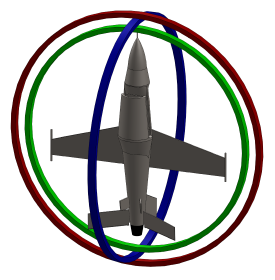
\includegraphics[width=0.9\textwidth]{figs/gimbal-lock}
\caption{Locked gimbal with loss of DOF}
\label{fig:gimbal-lock}
\end{subfigure}
\caption{Mechanical gimbal lock}
\vspace{-15pt}
\end{figure} 
\par
What is clear physically is not necessarily as obvious mathematically. A loss of rank occurs in the Euler Matrix $\Psi(\eta)$, defined previously in Eq:\ref{eq:angular-rates.e} from Sec:\ref{subsec:proto.conventions.frames}. That relation between angular velocity, in the inertial frame or inversely in the body frame, and the angular rates of the Euler Angles has a determinant:
\begin{equation}\label{eq:euler-derivative}
\begin{bmatrix}
\dot{\phi}\\
\dot{\theta}\\
\dot{\psi}
\end{bmatrix}
=\begin{bmatrix}
1 & sin(\phi)tan(\theta) & cos(\phi)tan(\theta)\\
0 & cos(\phi) & -sin(\phi)\\
0 & sin(\phi)sec(\theta) & cos(\phi)sec(\theta)\\
\end{bmatrix}
\begin{bmatrix}
p\\
q\\
r
\end{bmatrix}
=\Phi(\eta)\omega_b
\end{equation}
\vspace{-2pt}
\begin{equation}
\rightarrow det\big(\Phi(\eta)\big)=cos(\phi)\big(cos(\phi)sec(\theta)\big)+sin(\phi)\big(\sin(\phi)sec(\theta)\big)=sec(\theta)
\end{equation}
\vspace{-6pt}
\begin{equation}
\therefore \underset{{\theta \rightarrow \pi /2}}{lim}|\Phi(\eta)|=sec(\theta)\rightarrow \infty
\end{equation}
The Euler matrix $\Phi(\eta)$ looses rank as $\theta\rightarrow\pi/2$, loosing differentiability as well. The physical consequence of this is the loss of a degree of freedom. More specifically, if one looks at how the Z-Y-X rotation (or transformation) matrices are formulated, from Eq:\ref{eq:rotationmatrix}.
\begin{subequations}
\begin{equation}
R_I^b = R_zR_yR_x=\begin{bmatrix}
c_\psi & -s_\psi & 0\\
s_\psi & c_\psi & 0\\
0 & 0 & 1
\end{bmatrix}
\begin{bmatrix}
c_\theta & 0 & s_\theta\\
0 & 1 & 0\\
-s_\theta & 0 & c_\theta
\end{bmatrix}
\begin{bmatrix}
1 & 0 & 0\\
0 & c_\phi & -s_\phi\\
0 & s_\phi & c_\phi
\end{bmatrix}
\end{equation}
\begin{equation}
R_I^b(\eta)=\begin{bmatrix}
c_\psi c_\theta & c_\psi s_\theta s_\phi - s_\psi c_\phi & c_\psi s_\theta c_\phi + s_\psi s_\phi\\
s_\psi c_\theta & s_\psi s_\theta s_\phi + c_\psi c_\phi & s_\psi s_\theta  c_\phi - c_\psi s_\phi\\
-s_\theta & c_\theta s_\phi & c_\phi c_\theta\\
\end{bmatrix}
\end{equation}
In the case where $\theta=\pi/2$, and using trigonometric double angles, the following can be reduced;
\begin{equation}
R_I^b(\eta)=\begin{bmatrix}
0 & c_\psi s_\phi - s_\psi c_\phi & c_\psi c_\phi + s_\psi s_\phi\\
0 & s_\psi s_\phi + c_\psi c_\phi & s_\psi c_\phi - c_\psi s_\phi\\
-1 & 0 & 0\\
\end{bmatrix}\Bigg|_{\theta=\pi/2}
\end{equation}
\vspace{-6pt}
\begin{equation}
=
\begin{bmatrix}
0 & s(\phi - \psi) & c(\phi - \psi)\\
0 & c(\phi - \psi) & s(\phi - \psi)\\
-1 & 0 & 0
\end{bmatrix}
\end{equation}
\vspace{-4pt}
\begin{equation}\label{eq:gimbal}
=R_{x'}(\phi-\psi)
\end{equation}
\end{subequations}
Where the resultant in Eq:\ref{eq:gimbal} represents an $\hat{X}'$-axis rotation in a new intermediate frame, post a $\pi/2$ rotation about the $\hat{Y}$-axis. Through trigonometric double angles a degree of freedom is lost at $\theta=\pi/2$, when $\phi$ \& $\psi$ effect the same angle.
%====================================================
\subsection{Quaternion Dynamics}
\label{subsec:dynamics.rigidbody.quaternion}
%====================================================
An algorithm proposed in \cite{euleranglesingularity} suggested a solution to avoid Euler Angle singularities. The heuristic proposed involved switching between sequence conventions (ZYX,ZYZ etc\ldots there are 12 in total) such that the singularity is always avoided. However the implementation of such an algorithm is cumbersome and inefficient. Far more elegant is the use of \emph{quaternion} attitude representations in $\mathbb{R}^4$ (\cite{rotationsequences,quaterniondynamics,spacecraftattitutdequaternions} amongst others\ldots most notably made popular by \cite{shoemake} for use in animation).
\par
A quaternion is analogous to a rotation matrix because it represents an attitude difference between two reference frames. An $\mathbb{R}^3$ attitude is paramterized as one rotation $\theta$ about a single unit \emph{Euler} axis $\hat{u}$ (demonstrated using the Rodriguez Formula in \cite{unwinding}). In brief a quaternion consists of a scalar component, $q_0$, and complex vector component, $\vec{q}\in \mathbb{C}^3$, such that;
\begin{equation}
Q\triangleq 
\begin{bmatrix}
q_0 \\
\vec{q}
\end{bmatrix}
~~\in\mathbb{R}^4
\end{equation}
The relationship between an Euler Angles rotation matrix $R_I^b(\eta)$ and a quaternion attitude $Q_b$ is given by the Rodriguez formula:
\begin{equation}\label{eq:rodriguez}
R_I^b(\eta)=R(Q_b)=\mathbb{I}+2q_0[\vec{q}\hspace{2pt}]_\times+2[\vec{q}\hspace{2pt}]_\times\text{}^2
\end{equation}
Where $[.]_\times$ is the cross-product matrix defined earlier in Eq:\ref{eq:cross-product-matrix}. All quaternions, unless otherwise specified, are unit quaternions $Q\in\mathbb{Q}_u$. Quaternion with a unity magnitude ensure that rotational operations maintain the vector operand's magnitude. A unit quaternion is defined:
\begin{equation}
\norm{Q}=\sqrt{{q_0}^2+\vec{q}\text{}\hspace{2pt}^2}=1
\end{equation}
Quaternion multiplication is distributive and associative, but not commutative. Specifically a quaternion multiplciation operation is equivalent to the Hamilton product. For two quaternions, $Q$ \& $P$:
\begin{subequations}
\begin{equation}
Q\otimes P = \begin{bmatrix}
q_0 \\
\vec{q}
\end{bmatrix}
\otimes
\begin{bmatrix}
p_0 \\
\vec{p}
\end{bmatrix}
\end{equation}
\vspace{-5pt}
\begin{equation}
=\begin{bmatrix}
q_0p_0-\vec{q}\cdot\vec{p}\\
q_0\vec{p}+p_0\vec{q}+\vec{q}\times\vec{p}
\end{bmatrix}
\end{equation}
\vspace{-5pt}
\begin{equation}\label{eq:quaternion-product}
=q_0 p_0 - \vec{q}\cdot \vec{p}+p_0 \vec{q} + q_0 \vec{p} + \vec{q}\times\vec{p}
\end{equation}
\end{subequations}
Because the vector component of a quaternion is complex valued, it is natural that there exists a quaternion complex conjugate property, defined as:
\begin{equation}
Q^*=\begin{bmatrix}
q_0 \\
-\vec{q}
\end{bmatrix}
\end{equation}
It then follows that the fundamental quaternion identity is:
\begin{equation}
Q\otimes Q^* = \mathbb{I}_{4\times 4}
\end{equation}
A right handed quaternion rotation applied to a vector $\vec{v} \in\mathbb{R}^3$ involves multiplication by two unit quaternions. 
\begin{equation}
\begin{bmatrix}
0 \\
\vec{v}\hspace{2pt}'
\end{bmatrix}
=Q\otimes
\begin{bmatrix}
0 \\
\vec{v}
\end{bmatrix}
\otimes Q^*
\end{equation}
Mostly, the zero scalar components are omitted in a rotation (\emph{or transformation}) operation, it is implied that vector operands are substituted with quaternions.
\begin{equation}\label{eq:quaternion-rotation}
\vec{v}\hspace{2pt}'=Q \otimes (\vec{v}\hspace{2pt}) \otimes Q^*
\end{equation} 
In the case of rigid body attitude parameterization with quaternions, $Q_b$ is the quaternion which represents the difference between $\mathcal{F}^b$ and $\mathcal{F}^I$. A quaternion operator is equivalent to a rotation matrix operation, for some vector $\vec{v}_I\in\mathcal{F}^I$;
\begin{equation}
\vec{v}_b=R_I^b(\eta)\vec{v}_I \underset{Q}{\iff} Q_b \otimes (\vec{v}_I) \otimes Q_b^*
\end{equation}
Since quaternions are non-commutative, the construction of a body quaternion $Q_b$ from an Euler angle set $\vec{\eta}$ is sequence dependent. Euler angles, despite being singular, are conceptually simple terms for describing a body's orientation. A Z-Y-X sequenced body quaternion, $Q_b$, can be constructed from Euler angles as:
\begin{equation}\label{eq:quaternion-sequence}
Q_b=Q_z\otimes Q_y\otimes Qx=\begin{bmatrix}
cos(\psi/2)\\
0\\
0\\
sin(\psi/2)
\end{bmatrix}
\otimes
\begin{bmatrix}
cos(\theta/2)\\
0\\
sin(\theta/2)\\
0
\end{bmatrix}
\otimes
\begin{bmatrix}
cos(\phi/2)\\
sin(\phi/2)\\
0\\
0
\end{bmatrix}
\end{equation}
A quaternion time derivative, defined in \cite{quaterniondynamics}, with $Q_\omega$ being a quaternion with a vector component equal to angular velocity $\vec{\omega}_{b/I}$ and a zero scalar component, is:
\begin{equation}\label{eq:quaternion-deriv}
\frac{d}{dt}Q_b=\frac{1}{2}Q_b\otimes Q_{\omega}=\begin{bmatrix}
-\frac{1}{2}\vec{q}\hspace{2pt}^{T} \vec{\omega}_b\\
\frac{1}{2}\big([\vec{q}\hspace{2pt}]_\times+q_0\mathbb{I}\big)\vec{\omega}_b
\end{bmatrix}
\end{equation}
Using quaternions to represent attitudes negates the need for an Euler Matrix, $\Phi(\eta)$, to represent attitudes and their rates. A body quaternion is fully defined in the inertial frame with respect to the body frame or inversely so. The first quaternion time derivative replaces angular velocity rate differentials Eq:\ref{eq:states.a} and Eq:\ref{eq:states.c};
\begin{subequations}
\begin{equation}
\dot{\mathcal{E}}=R_b^I(-\eta)\vec{\nu}\underset{Q}{\iff}Q_b(-\eta)\otimes\vec{\nu}\otimes Q_b(-\eta)^*=Q_b^*\otimes \vec{\nu} \otimes Q_b~~~~\in\mathcal{F}^I
\end{equation}
\vspace{-14pt}
\begin{equation}
\dot{\eta}=\Phi(\eta)\vec{\omega}_b~~\in\mathcal{F}^{v2,v1,I}\underset{Q}{\iff}\dot{Q}_b=\frac{1}{2}Q_b\otimes Q_\omega~~\in\mathcal{F}^{I}
\end{equation}
\end{subequations}
Second order time derivatives for quaternion acceleration aren't as useful or concise as their higher order velocity counterparts. The second order derivative is provided here however it's only relevant to quaternion backstepping later in the control chapter. If possible, quaternion accelerations are mostly avoided due to their complexity of their evaluation;
\begin{equation}
\ddot{Q}\big(\dot{Q},Q,t)=\dot{Q}\otimes Q^* \otimes \dot{Q}+\frac{1}{2}Q\otimes \big[J_b^{-1}(\tau-4(Q^*\otimes \dot{Q})\times(J_b(Q^*\otimes \dot{Q}))\big]
\end{equation}
An Euler angle attitude error state used for control plants is defined as the subtracted error between desired and existing attitude orientations $\vec{eta}_d$ and $\vec{eta}_b$ respectively. Where $\vec{\eta}_d$ is some attitude produced from a trajectory generation loop.
\begin{equation}\label{eq:euler-error}
\vec{\eta}_e=\vec{\eta}_d-\vec{\eta}_b
\end{equation}
In contrast with Eq:\ref{eq:euler-error}, a quaternion attitude error is a multiplicative term defined as the difference between two quaternions $Q_d$ and $Q_b$;
\begin{equation}\label{eq:quaternion-error}
Q_e=Q_d^*\otimes Q_b
\end{equation}
Quaternion attitude control and its stability goals are expanded upon later in Sec:\ref{subsec:control.attitude.problem}.
%====================================================
\subsection{Quaternion Unwinding}
\label{subsec:dynamics.rigidbody.unwinding}
%====================================================
Although quaternions are indeed better than Euler angles, lacking the associated singularity, they do contain one caveat. Becuase a quaternion $Q=[q_0~\vec{q}\hspace{2pt}]^T$ represents a body's attitude in $\mathbb{R}^3$ using $\mathbb{R}^4$ there is an infinite coverage of attitude states, \cite{unwinding}. Each unit quaternion, stemming from Euler-Rodriguez theorem, represents a single Euler-axis rotation of $\theta$ about a unit axis $\hat{u}$ such that:
\begin{equation}
Q=\begin{bmatrix}
q_0\\
\vec{q}
\end{bmatrix}=
\begin{bmatrix}
cos(\theta/2)\\
sin(\theta/2)\hat{u}
\end{bmatrix}
\end{equation}
That rotation is applied with a quaternion operator, Eq:\ref{eq:quaternion-rotation}. For every attitude state in 3-Dimensions there exist two unique quaternions which correspond to the same orientation, differing by their rotational direction about the Euler-axis. The rotation angle $\theta$ about the Euler-axis $\hat{u}$ is reciprocal in that $\theta=\theta + 2k\pi,~k\in\mathbb{N}$, there are then two definitions for $Q_b$;
\begin{subequations}
\begin{equation}
Q_b =
\begin{bmatrix}
q_0 \\
\vec{q}
\end{bmatrix}
=
\begin{bmatrix}
cos(\theta/2)\\
sin(\theta/2)\hat{u}
\end{bmatrix}
\end{equation}
\vspace{-6pt}
\begin{equation}
Q_b=\begin{bmatrix}
cos(\pi - \theta/2)\\
sin(\pi - \theta/2)\hat{u}
\end{bmatrix}
=
\begin{bmatrix}
-cos(\theta/2)\\
sin(\theta/2)\hat{u}
\end{bmatrix}
\end{equation}
\vspace{-6pt}
\begin{equation}\label{eq:euler-quaternion}
\eta\in\mathbb{R}^3\underset{Q}{\iff}\begin{bmatrix}
\pm q_0\\
\vec{q}
\end{bmatrix}
\in\mathbb{R}^4
\end{equation}
\end{subequations}
Eq:\ref{eq:euler-quaternion} asserts that for each attitude in $\mathbb{R}^3$ there are \emph{two} corresponding quaternions in $\mathbb{R}^4$; $[\pm q_0~\vec{q}~]^T$. A consequence of this is two possible error state trajectories exist for every attitude difference. Both a clockwise, $\theta$, and an anticlockwise, $2\pi-\theta$, rotations which point to the same quaternion attitude error state. This could lead to an erroneous and unnecessary "unwinding" of a complete counter revolution. As such for attitude controllers the requirement is that for positive and negative scalars the control input is consistent:
\begin{equation}
\vec{\nu}_d=h([q_0~\vec{q}\hspace{2pt}]^T,t)=h([-q_0~\vec{q}\hspace{2pt}]^T,t)
\end{equation}
Or more simply that $Q_e=[|q_0|~\vec{q}\hspace{2pt}]^T$. The most simple solution adhering to that constraint, which is often used, is to neglect the quaternion scalar component altogether. Using a reduced error state, only the quaternion error vector as an argument for the control law; $h(\vec{q}_e,t)$. Such a solution is an oversimplification and would only ever be locally stable. 
\par
An alternative is to use only the absolute quaternion scalar, which ensures the error state represents a right-handed (clockwise) rotation and not necessarily the shortest path. If the resolution of trajectory co-ordinates generated is sufficiently fine the control plant won't encounter a problem. One proposal presented in \cite{nonlinearquadcopter} suggested using a \emph{signum} operator to design the controller coefficient sign for the virtual angular velocity, $\vec{\omega}_d$ control plant input. 
\begin{subequations}\label{eq:signum-unwinding}
\begin{equation}
\vec{\omega}_d=\frac{2}{\Gamma_1}sgn(q_0)\vec{q}
\end{equation}
\begin{equation}
sgn(q_0)=
\begin{cases}\begin{array}{ll}
1 & ~~q_0\geq 0\\
-1 & ~~q_0< 0\\
\end{array}
\end{cases}
\end{equation}
\end{subequations}
Eq:\ref{eq:signum-unwinding} was shown to be asymptotically stable but only locally in the case where the Euler-axis angle is constrained; $\theta\leq \pm\pi$. That control law  would still need the control torques to be calculated from that angular velocity $\vec{\omega}_d$ setpoint.
\par
In \cite{intelligentbackstep}, the authors used a backstepping controller with a trajectory using the absolute quaternion scalar. The resultant was a global asymptotically stable control law which tracked quaternion setpoints for a satellite's attitude. Controllers presented in Sec:\ref{sec:control.attitude} all incorporate the signed quaternion scalars into the control law;  hence relying on the trajectory generation to provide the desired direction of the rotation path.
%====================================================
\section{Multibody Nonlinearities}
\label{sec:dynamics.nonlinearities}
%====================================================
Typically multibody dynamics are solved (and simulated) as a series of constrained torque and force responses. There are different schools of thought on the subject which each propose methodologies for stepping through the systems dynamics (\emph{e.g} Implicit Euler integration;\cite{physicallybased,multibodydynamics}\ldots). For the prototype under consideration, only relative rotational motion is mechanically permissible between the connected rigid bodies. Each body is considered independently whose constraint torques induced from excitation are imposed onto sequential rotational joints. Opposing those torques are \emph{gyroscopic} and \emph{inertial} Newtonian responses. Those responses are now quantified and introduced to the dynamic model derived in Sec:\ref{subsec:dynamics.rigidbody.lagrange}. The design has no translational degrees of freedom between each body and is treated as rigid.
\par
A distinction must be made between torque responses here and those previously in Eq:\ref{eq:states.d}. The torque term(s) previously regard the entire body as rigid, the induced responses are then as a result of the entire multibody's collective motion. The following is with regards to the internal relative movements between each body. The analysis here aims to approximate the highly non-linear dynamic system as clear responses induced from servo rotations of inner and middle ring bodies, $\Delta\lambda_i$ and $\Delta\alpha_i$ respectively.
\par
Alternatively the net dynamics could be derived from a Lagrangian for the \emph{entire} 13 body dynamic system. Where those connected bodies are; four rotor/propeller bodies (Fig:\ref{fig:inertia-prop}), four inner ring bodies (Fig:\ref{fig:inertia-inner}), four middle ring bodies (Fig:\ref{fig:inertia-middle}) and finally the frame structure (Fig:\ref{fig:inertia-frame}) each with 6 degrees of freedom. The constraints on the assembly's joints would reduce the degrees of freedom and simplify solving for net responses. However such an approach is not used here as complete 6-DOF equations for every rigid body first need to be quantified before they can be reduced, making the kinematic derivation dramatically more cumbersome.
\par
\emph{\color{gray}Rotation matrices are used in the following derivations owing to the fact that induced torque responses are dependent on transformed rotational inertias. Quaternions, as mentioned in Sec:\ref{sec:proto.inertia}, are ill-suited to inertia transformations. Moreover each actuating servo has a range of $\pm\pi/2$ so rotation matrix singularities won't be a concern\ldots}
%====================================================
\subsection{Relative Rotational Gyroscopic \& Inertial Torques}
\label{subsec:dynamics.nonlinearities.gyrotorques}
%====================================================
The torque responses induced by relative rotations, the only permissible intra-body movement, are transferred from the interacting bodies as a result of Newton's second law applied to rotational motion. For each of the motor modules' pitching or rolling motion the respective servo motors apply some torque to invoke that rotation. Opposed to that angular acceleration are both inertial and gyroscopic torque responses of the body being rotated.
\par
Each of the four motor modules are symmetrical and as such the induced torque response characteristics for one module can be extrapolated through a $\hat{Z}_b$ reference frame rotation. Each motor module is positioned relative to the body frame center of motion $\vec{\mathbf{O}}_b$ as in Fig:\ref{fig:body-frame}. Because each relative rotation from the actuator set, $u\in\mathbb{U}$, is actuated separately and upon a different body, their responses are calculated independently too.
\par
Drawing again from Lagrangian theory and considering only the angular kinetic for the inner ring assembly $\mathcal{F}^{M_i}$. There is no relative translational motion between each body and so there is no translational kinetic energy contribution. The translational kinetic energy for each module is an extension of body's kinetic energy in Eq:\ref{eq:3.7a} and independent of any actuator positions. The motor module's translational motion is accounted for in Eq:\ref{eq:rigid-frame.a}. 
\newpage
\begin{figure}
\centering
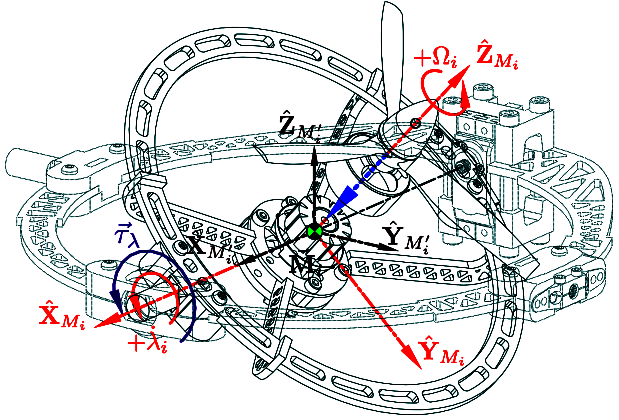
\includegraphics[width=0.6\textwidth]{figs/response-inner}
\caption{Exploded inertial bodies for $\vec{\tau}_\lambda$}
\label{fig:response-inner}
\end{figure}
Deriving dynamic responses for changes in $\lambda_i$ on the inner ring frame $\mathcal{F}^{M_i}$ relative to the middle ring frame $\mathcal{F}^{M_i'}$ requires a relative path co-ordinate to be defined. Seeing that the only path variable between the two frames is $\lambda_i$; the path co-ordinates $\vec{\mathbf{u}}(t)=\begin{bmatrix}\lambda_i&0&0\end{bmatrix}^T$ for the servo position $\lambda$ are used to form the Lagrangian for the inner ring's motion in the middle ring frame; $\mathcal{L}_{M_i'}\in\mathcal{F}^{M_i'}$. The inner ring assembly consists of two separate bodies (Fig:\ref{fig:response-inner}) with relative rotational motion and independent kinetic energies; the rotor assembly with an inertia $J_{r}$ (defined earlier in Eq:\ref{eq:prop-inertia}) and the inner ring (\emph{sans} rotor assembly) which has an inertia $J_{ir}$:
\begin{equation}
J_{ir}=J_{n}-J_{r}=J_{M_i}-J_{r}~~~~\in\mathcal{F}^{M_i}
\end{equation} 
Where $J_{M_i}$ is the net inertia for the inner ring assembly from Eq:\ref{eq:inertia.inner}. The rotor assembly has an angular velocity $\vec{\omega}_{r/M_i'}$ relative to the middle ring frame $\mathcal{F}^{M_i'}$:
\begin{subequations}\label{eq:angular-rot}
\begin{equation}
\vec{\omega}_{r/M_i'}=R_x(-\lambda)\vec{\Omega}_i+\frac{d}{dt}(\vec{\lambda}_i)~~~~\in\mathcal{F}^{M_i'}
\end{equation}
\vspace{-12pt}
\begin{equation}
=R_x(-\lambda)\vec{\Omega}_i+\dot{\vec{\lambda}}_i
\end{equation}
\end{subequations}
With propeller's angular velocity vector $\vec{\Omega}_i=\begin{bmatrix}0 & 0 & \Omega_i\end{bmatrix}^T$ in $[\text{rad.s}^{-1}]$, \underline{not in revolutions per second}, and the servo position $\vec{\lambda}_i=\begin{bmatrix}\lambda_i & 0 & 0\end{bmatrix}^T$. Similarly the inner ring's angular velocity $\vec{\omega}_{M_i/M_i'}$ relative to $\mathcal{F}^{M_i'}$ is only as a result of $\Delta\lambda_i$:
\begin{equation}\label{eq:angular-inner}
\vec{\omega}_{M_i/M_i'}=\frac{d}{dt}(\vec{\lambda}_i)=\dot{\vec{\lambda}}_i~~~~\in\mathcal{F}^{M_i'}
\end{equation}
The Lagrangian for the inner ring's energy $\mathcal{L}_{M_i'}$, relative to the middle ring frame $\mathcal{F}^{M_i'}$, consists purely of rotational kinetic energy from Eq:\ref{eq:angular-rot} and Eq:\ref{eq:angular-inner}. Both inertias for the rotor and inner ring bodies, $J_r$ and $J_{ir}$ respectively, are transformed onto the middle ring frame $\mathcal{F}^{M_i'}$:
\begin{subequations}
\begin{equation}
\mathcal{L}_{M_i'}=\frac{1}{2}\vec{\omega}_{r/M_i'}\text{}^T\big(J_{r}'\big)\vec{\omega}_{r/M_i'}+\frac{1}{2}\vec{\omega}_{M_i/M_i'}\text{}^T\big(J_{ir}'\big)\vec{\omega}_{M_i/M_i'}
\end{equation}
\vspace{-12pt}
\begin{equation}\label{eq:lagrange-inner}
=\frac{1}{2}\Big(R_x(-\lambda)\vec{\Omega}_i+\dot{\vec{\lambda}}_i\Big)^T\big(R_x(\lambda)\big(J_{r}\big)R_x^{-1}(\lambda)\big)\Big(R_x(-\lambda)\vec{\Omega}_i+\dot{\vec{\lambda}}_i\Big)+\frac{1}{2}\dot{\vec{\lambda}}_i^{\hspace{2pt}T}\big(R_x(\lambda)\big(J_{ir}\big)R_x^{-1}(\lambda)\big)\dot{\vec{\lambda}}_i
\end{equation}
\end{subequations}
Noting that the inner ring's inertia $J_{ir}$ is now a separate body from the rotor $J_{r}$. Recalling the Euler-Lagrange formulation from Eq:\ref{eq:euler-lagrange} with path co-ordinates $\vec{\mathbf{u}}(t)$ for the inner ring frame, $\mathcal{F}^{M_i}$, relative to  the middle ring frame, $\mathcal{F}^{M_i'}$:
\begin{equation}
\frac{d}{dt}\bigg(\frac{\delta \mathcal{L}_{M_i'}}{\delta \dot{\vec{\mathbf{u}}}}\bigg)-\frac{\delta \mathcal{L}_{M_i'}}{\delta \vec{\mathbf{u}}} = \vec{\mathbf{U}} = \vec{\tau}_{\lambda}~~~~\in\mathcal{F}^{M_i'}
\end{equation}
From \cite{rotationlinearize} the partial derivative of a rotation matrix $R_x(\lambda)$ (and by extension the \emph{transformation matrix} $R_x(-\lambda)$) is linearized using Taylor series expansion. It follows that for some small perturbation $\delta\theta$ away from the nominal $\bar{\theta}$, a generalized rotation matrix about an axis $\hat{u}$ by that angle $\theta$ becomes a first order approximation:
\begin{equation}\label{eq:rotation-linear}
R_u(\bar{\theta}+\delta\theta)\approx\underbrace{\big(1-[\Psi_u(\bar{\theta})\delta\theta]_\times\big)}_{\text{infinitesimal rot}}R_u(\bar{\theta})
\end{equation}
Where $\Psi_u(\theta)$ is a generalized Euler matrix derivative analogous to Eq:\ref{eq:angular-rates.c}. The consequence of Eq:\ref{eq:rotation-linear} is that, for the transformed rotational inertias in Eq:\ref{eq:lagrange-inner}, both $R_x(\lambda)^T\big(J_r\big)R_x(\lambda)$ and $R_x(\lambda)^T\big(J_{ir}\big)R_x(\lambda)$ can be approximated using their instantaneous transformation with no partial rate derivatives.
\begin{subequations}
\begin{equation}
R_x(\lambda)\big(J_r\big)R_x^{-1}(\lambda)=J_r'\rightarrow \frac{\delta}{\delta\vec{\mathbf{u}}} J_r' = \frac{\delta}{\delta\lambda_i}J_r'\approx 0
\end{equation}
Similarly for the inner ring without the rotor body's contribution:
\begin{equation}
R_x(\lambda)\big(J_{ir}\big)R_x^{-1}(\lambda)=J_{ir}'\rightarrow \frac{\delta}{\delta\vec{\mathbf{u}}} J_{ir}' = \frac{\delta}{\delta\lambda_i}J_{ir}'\approx 0
\end{equation}
\end{subequations}
It follows that the partial derivatives of the Lagrangian Eq:\ref{eq:lagrange-inner} with respect to $\vec{\mathbf{u}}$ are negligible; $\delta\mathcal{L}_{M_i'}/\delta\vec{\mathbf{u}}=0$. Only the partial derivative with respect to the path derivative $\dot{\vec{\mathbf{u}}}$ remains. That partial derivative is then:
\begin{subequations}
\begin{equation}\label{eq:3.42b}
\therefore\frac{\delta \mathcal{L}_{M_i'}}{\delta \dot{\vec{\mathbf{u}}}}=\big(J_{r}'\big)\Big(R_x(-\lambda)\vec{\Omega}_i+\dot{\vec{\lambda}}_i\Big)+\big(J_{ir}'\big)\dot{\vec{\lambda}}_i
\end{equation}
Inserting the Reynolds transportation theorem, Eq:\ref{eq:reynolds} for a vector's derivative in a rotating reference frame, into Eq:\ref{eq:3.42b} yields:
\begin{multline}
\rightarrow \frac{d}{dt} \bigg(\frac{\delta \mathcal{L}_{M_i'}}{\delta \dot{\vec{\mathbf{u}}}}\bigg)=\Big(\big(J_{r}'\big)R_x(-\lambda)\dot{\vec{\Omega}}_i+\vec{\omega}_{M_i/M_i'}\times \big(J_{r}'\big)R_x(-\lambda)\vec{\Omega}_i+\big(J_{r}'\big)\ddot{\vec{\lambda}}_i+\vec{\omega}_{M_i/M_i'}\times \big(J_{r}'\big)\dot{\vec{\lambda}}_i\Big)\\+\Big(\big(J_{ir}'\big)\ddot{\vec{\lambda}}_i+\vec{\omega}_{M_i/M_i'}\times \big(J_{ir}'\big)\dot{\vec{\lambda}}_i\Big)
\end{multline}
\end{subequations}
Recombining inertial contributions with the same angular velocity ($J_{r}'+J_{ir}'=J_{n}'$) and recognizing that, from Eq:\ref{eq:angular-inner} $\vec{\omega}_{M_i/M_i'}=\dot{\vec{\lambda}}$; the generalized net torque encountered by a rotation of $\lambda$ is:
\begin{subequations}
\begin{equation}
\vec{\tau}_\lambda=\frac{d}{dt}\bigg(\frac{\delta\mathcal{L}_{M_i'}}{\delta\dot{\vec{\mathbf{u}}}}\bigg)=\big(J_{r}'\big)\dot{\vec{\Omega}}_i\text{}\hspace{-2pt}'+\dot{\vec{\lambda}}_i\times \big(J_{r}'\big)\vec{\Omega}_i\text{}\hspace{-2pt}'+\big(J_{n}'\big)\ddot{\vec{\lambda}}_i+\dot{\vec{\lambda}}_i\times \big(J_{n}'\big)\dot{\vec{\lambda}}_i~~~~\in\mathcal{F}^{M_i'}
\end{equation}
Using $\vec{\Omega}_i\text{}\hspace{-2pt}'$ and $\dot{\vec{\Omega}}_i\text{}\hspace{-2pt}'$ as the respective transformed angular velocity and acceleration of the propeller in the middle ring frame;
\begin{equation}
\vec{\Omega}_i\text{}\hspace{-2pt}'=R_x(-\lambda)\vec{\Omega}_i~~~~\in\mathcal{F}^{M_i'}
\end{equation}
\vspace{-10pt}
\begin{equation}
\dot{\vec{\Omega}}_i\text{}\hspace{-2pt}'=R_x(-\lambda)\dot{\vec{\Omega}}_i~~~~\in\mathcal{F}^{M_i'}
\end{equation}
\end{subequations}
The net torque response from a $\lambda_i$ rotation, induced in the middle ring frame $\mathcal{F}^{M_i'}$, can be grouped into second order \emph{inertial} and first order \emph{gyroscopic} components;
\begin{equation}\label{eq:torque-induced-inner}
\vec{\tau}_\lambda=\underbrace{\big(J_r'\big)\dot{\vec{\Omega}}_i\text{}\hspace{-2pt}'+\big(J_{M_i}'\big)\ddot{\vec{\lambda}}_i}_{Inertial}+\underbrace{\dot{\vec{\lambda}}_i\times \big(J_r'\big)\vec{\Omega}_i\text{}\hspace{-2pt}'+\dot{\vec{\lambda}}_i\times \big(J_{M_i}'\big)\dot{\vec{\lambda}}_i}_{Gyroscopic}~~~~\in\mathcal{F}^{M_i'}
\end{equation}
Taking special care not to confuse $J_{n}'$ and $J_{m}$. The former being the inner ring's inertia transformed into the middle ring frame $\mathcal{F}^{M_i'}$ and the latter is the middle ring's inertia in that same reference frame. 
\par
Similarly for the middle ring frame $\mathcal{F}^{M_i'}$ relative to the intermediary frame $\mathcal{F}^{M_i''}$, the only relative path variable is $\vec{\mathbf{v}}(t)=\begin{bmatrix}0 & \alpha_i & 0\end{bmatrix}^T$. The entire motor module structure consists of three separate rotating bodies each with their own relative angular velocities; the rotor assembly, inner ring structure and middle ring structure (Fig:\ref{fig:response-middle}).
\par
\begin{figure}
\centering
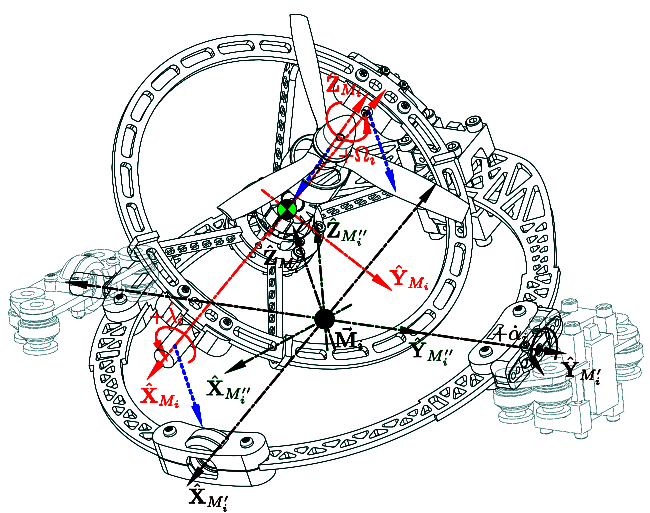
\includegraphics[width=0.6\textwidth]{figs/response-middle}
\caption{Exploded inertal bodies for $\vec{\tau}_{\alpha}$}
\label{fig:response-middle}
\end{figure}
Following the same process to evaluate the middle ring's response, but with respect to the intermediary frame $\mathcal{F}^{M_i''}$. The rotor assembly has a transformed inertia:
\begin{subequations}
\begin{equation}
J_r''=R_y(\alpha)\big(J_r'\big)R_y^{-1}(\alpha)=R_y(\alpha)R_x(\lambda)\big(J_r\big)R_x^{-1}(\lambda)R_y^{-1}(\alpha)~~~~\in\mathcal{F}^{M_i''}
\end{equation}
The inner ring has an inertia, still \emph{without} including the rotor assembly:
\begin{equation}
J_{ir}''=R_y(\alpha)\big(J_{ir}'\big)R_y^{-1}(\alpha)=R_y(\alpha)R_x(\lambda)\big(J_{ir}\big)R_x^{-1}(\lambda)R_y^{-1}(\alpha)~~~~\in\mathcal{F}^{M_i''}
\end{equation} 
Lastly the middle ring assembly's inertia from Eq:\ref{eq:inertia.middle.a}, with neither the rotor's nor the inner ring's contributions:
\begin{equation}
J_m'=R_y(\alpha)\big(J_{\zeta}\big)R_y^{-1}(\alpha)-R_y(\alpha)R_x(\lambda)\big(J_\text{n}\big)R_x^{-1}(\lambda)R_y^{-1}(\alpha)
\end{equation}
\vspace{-10pt}
\begin{equation}
=J_{\zeta}'-J_{n}''=J_{\zeta}'-\big(J_{ir}''+J_{r}''\big)~~~~\in\mathcal{F}^{M_i''}
\end{equation}
\end{subequations}
Where $J_{\zeta}$ is the collective motor module inertia from Eq:\ref{eq:inertia.middle.b}. Each body then has its own relative angular velocity with respect to the frame $\mathcal{F}^{M_i''}$. For the rotor; $\vec{\omega}_{r/M_i''}$ is the relative angular velocity of that assembly:
\begin{subequations}\label{eq:rotor-relative}
\begin{equation}
\vec{\omega}_{r/M_i''}=R_y(-\alpha)R_x(-\lambda)\vec{\Omega}_i+\frac{d}{dt}\Big(R_y(-\alpha)\vec{\lambda}_i\Big)+\frac{d}{dt}\big(\vec{\alpha}_i\big)~~~~\in\mathcal{F}^{M_i''}
\end{equation}
\vspace{-10pt}
\begin{equation}
=R_y(-\alpha)R_x(-\lambda)\vec{\Omega}_i+R_y(-\alpha)\dot{\vec{\lambda}}_i+\dot{\vec{\alpha}}_i
\end{equation}
\vspace{-10pt}
\begin{equation}
\rightarrow \vec{\omega}_{r/M_i''}=\vec{\Omega}_i\text{}\hspace{-2pt}''+\dot{\vec{\lambda}}_i\text{}\hspace{-2pt}'+\dot{\vec{\alpha}}_i
\end{equation}
\end{subequations}
Next, the inner ring has an angular velocity $\vec{\omega}_{M_i/M_i''}$ relative to the intermediate frame $\mathcal{F}^{M_i''}$:
\begin{subequations}\label{eq:inner-relative}
\begin{equation}
\vec{\omega}_{M_i/M_i''}=\frac{d}{dt}\big(R_y(-\alpha)\vec{\lambda}_i\big)+\frac{d}{dt}(\vec{\alpha}_i)~~~~\in\mathcal{F}^{M_i''}
\end{equation}
\vspace{-10pt}
\begin{equation}
=R_y(\alpha)\dot{\vec{\lambda}}_i+\dot{\vec{\alpha}}_i=\dot{\vec{\lambda}}_i\text{}\hspace{-2pt}'+\dot{\vec{\alpha}}_i
\end{equation}
\end{subequations}
Finally the middle ring has an angular velocity $\vec{\omega}_{M_i'/M_i''}$ relative to the intermediary frame:
\begin{equation}\label{eq:middle-relative}
\vec{\omega}_{M_i'/M_i''}=\frac{d}{dt}(\vec{\alpha}_i)=\dot{\vec{\alpha}}_i~~~~\in\mathcal{F}^{M_i''}
\end{equation}
Then using the relative path co-ordinate $\vec{\mathbf{v}}(t)$ the Lagrangian $\mathcal{L}_{M_i''}$ can be constructed for the motor module relative to the frame $\mathcal{F}^{M_i''}$;
\begin{equation}\label{eq:alpha-lagrange}
\mathcal{L}_{M_i''}=\frac{1}{2}\vec{\omega}_{r/M_i''}^{\hspace{2pt}T}\big(J_{r}''\big)\vec{\omega}_{r/M_i''}+\frac{1}{2}\vec{\omega}_{M_i'/M_i''}^{\hspace{2pt}T}\big(J_{ir}''\big)\vec{\omega}_{M_i'/M_i''}+\frac{1}{2}\vec{\omega}_{M_i'/M_i''}^{\hspace{2pt}T}\big(J_{m}'\big)\vec{\omega}_{M_i'/M_i''}
\end{equation}
Therefore the Langragian from Eq:\ref{eq:alpha-lagrange} expands to:
\begin{multline}\label{eq:alpha-lagrange-two}
\mathcal{L}_{M_i''}=\frac{1}{2}\Big[R_y(-\alpha)R_x(-\lambda)\vec{\Omega}_i+R_y(-\alpha)\dot{\vec{\lambda}}_i+\dot{\vec{\alpha}}\Big]^T\big(J_r''\big)\Big[R_y(-\alpha)R_x(-\lambda)\vec{\Omega}_i+Ry(-\alpha)\dot{\vec{\lambda}}_i+\dot{\vec{\alpha}}_i\Big]\\
+\frac{1}{2}\Big[R_y(-\alpha)\dot{\vec{\lambda}}_i+\dot{\vec{\alpha}}_i\Big]^T\big(J_{ir}''\big)\Big[R_y(\alpha)\dot{\vec{\lambda}}_i+\dot{\vec{\alpha}}_i\Big]
+\frac{1}{2}\dot{\vec{\alpha}}_i^{\hspace{2pt}T}\big(J_m'\big)\dot{\vec{\alpha}}_i
\end{multline}
Again, justifying the rotation matrix linearization using Eq:\ref{eq:rotation-linear}, matrices $J_r''$, $J_{ir}''$ and $J_m'$ are all instantaneous transformed inertias. The Euler-Lagrange formulation then simplifies, with the partial derivative $\delta\mathcal{L}_{M_i''}/\delta\vec{\mathbf{v}}=0$, to:
\begin{equation}
\frac{d}{dt}\Bigg(\frac{\delta\mathcal{L}_{M_i''}}{\delta\dot{\vec{\mathbf{v}}}}\Bigg)-\frac{\delta\mathcal{L}_{M_i''}}{\delta\vec{\mathbf{v}}}=\frac{d}{dt}\Bigg(\frac{\delta\mathcal{L}_{M_i''}}{\delta\dot{\vec{\mathbf{v}}}}\Bigg)=\vec{\mathbf{V}}=\vec{\tau}_\alpha
\end{equation}
Finding the partial derivative of the Lagrangian $\mathcal{L}_{M_i''}$ with respect to $\dot{\vec{\mathbf{v}}}$ is then:
\begin{subequations}
\begin{equation}
\frac{\delta\mathcal{L}_{M_i''}}{\delta\dot{\vec{\mathbf{v}}}} = \big(J_r''\big)\Big[R_y(-\alpha)R_x(-\lambda)\vec{\Omega}_i+R_y(-\alpha)\dot{\vec{\lambda}}_i+\dot{\vec{\alpha}}_i\Big]+\big(J_{ir}''\big)\Big[R_y(-\alpha)\dot{\vec{\lambda}}_i+\dot{\vec{\alpha}}_i\Big]+\big(J_m'\big)\dot{\vec{\alpha}}_i
\end{equation}
\vspace{-12pt}
\begin{multline}\label{eq:alpha-lagrange-deriv}
\rightarrow \frac{d}{dt}\Bigg(\frac{\delta \mathcal{L}_{M_i''}}{\delta\dot{\vec{\mathbf{v}}}}\Bigg)=\Big(\big(J_r''\big)\dot{\vec{\Omega}}_i\hspace{-2pt}''+\vec{\omega}_{M_i/M_i''}\times\big(J_r''\big)\vec{\Omega}_i\hspace{-2pt}''+\big(J_r''\big)\ddot{\vec{\lambda}}_i\hspace{-2pt}'+\vec{\omega}_{M_i/M_i''}\times \big(J_r''\big)\dot{\vec{\lambda}}_i\hspace{-2pt}'+\big(J_r''\big)\ddot{\vec{\alpha}}_i\\+\vec{\omega}_{M_i'/M_i''}\times \big(J_r''\big)\dot{\vec{\alpha}}_i\Big)
+\Big(\big(J_{ir}''\big)\ddot{\vec{\lambda}}_i\hspace{-2pt}'+\vec{\omega}_{M_i/M_i''}\times\big(J_{ir}''\big)\dot{\vec{\lambda}}_i\hspace{-2pt}'+\big(J_{ir}''\big)\ddot{\vec{\alpha}}_i+\vec{\omega}_{M_i'/M_i''}\times\big(J_{ir}''\big)\dot{\vec{\alpha}}_i\Big)+\Big(\big(J_m'\big)\ddot{\vec{\alpha}}_i\\+\vec{\omega}_{M_i'/M_i''}\times\big(J_m'\big)\dot{\vec{\alpha}}_i\Big)
\end{multline}
Which is an ominous and seemingly complicated result to try expand and make sense of. However it can be simplified; recognizing that Eq:\ref{eq:alpha-lagrange-deriv} contains kinetic energies already introduced in Eq:\ref{eq:torque-induced-inner}, but transformed to the frame $\mathcal{F}^{M_i''}$. After some mathematics, Eq:\ref{eq:alpha-lagrange-deriv} can be simplified with responses pertinent to $\Delta\alpha_i$ and then the generalized force transformed response $R_y(-\alpha)\vec{\tau}_\lambda$:
\begin{multline}
\vec{\mathbf{V}}=\ddot{\vec{\alpha}}_i\big(J_r''\big)+\dot{\vec{\alpha}}_i\times \big(J_r''\big)\big[R_y(-\alpha)R_x(-\lambda)\vec{\Omega}_i\big]+\dot{\vec{\alpha}}_i\times \big(J_r''\big)\big[R_y(-\alpha)\vec{\dot{\lambda}}\big]+\dot{\vec{\alpha}}_i\times \big(J_r''\big) \dot{\vec{\alpha}}_i+\ddot{\vec{\alpha}}_i\big(J_{ir}''\big)\\+\dot{\vec{\alpha}}_i\times \big(J_{ir}''\big)\big[R_y(-\alpha)\dot{\vec{\lambda}}_i\big]+\dot{\vec{\alpha}}_i\times \big(J_{ir}''\big)\dot{\vec{\alpha}}_i+\big(J_m'\big)\ddot{\vec{\alpha}}_i+\dot{\vec{\alpha}}_i\times \big(J_m'\big)\dot{\vec{\alpha}}_i+R_y(-\alpha)\vec{\tau}_\lambda
\end{multline}
Which can be further simplified by introducing angular velocities; $\vec{\omega}_{r/M_i''}$ of the rotor relative to the intermediary frame from Eq:\ref{eq:rotor-relative}, $\vec{\omega}_{M_i/M_i''}$ of the inner ring relative to that intermediary frame $\mathcal{F}^{M_i''}$ from Eq:\ref{eq:inner-relative} and finally $\vec{\omega}_{M_i'/M_i''}$ of the middle ring relative to the fixed intermediate frame from Eq:\ref{eq:middle-relative}.
\begin{multline}
=\ddot{\vec{\alpha}}_i\big(J_r''\big)+\dot{\vec{\alpha}}_i\times \big(J_r''\big)\vec{\omega}_{r/M_i''}+\ddot{\vec{\alpha}}_i\big(J_{ir}''\big)+\dot{\vec{\alpha}}_i\times \big(J_{ir}''\big)\vec{\omega}_{M_i/M_i''}+\ddot{\vec{\alpha}}_i\big(J_m'\big)+\dot{\vec{\alpha}}_i\times \big(J_m'\big)\vec{\omega}_{M_i'/M_i''}\\+R_y(-\alpha)\vec{\tau}_\lambda~~~~\in\mathcal{F}^{M_i''}
\end{multline}
\end{subequations}
Isolating the torque response from $\Delta\alpha$, and again grouping inertial bodies with shared angular velocities together. The first and second order \emph{gyroscopic} and \emph{inertial} responses are then:
\begin{equation} \label{eq:torque-induced-middle}
\vec{\tau}_\alpha(\lambda_i)=\underbrace{\big(J_{\zeta}'(\lambda)\big)\ddot{\vec{\alpha}}_i}_{Inertial}+\underbrace{\dot{\vec{\alpha}}_i\times \big(J_r''\big)\vec{\omega}_{r/M_i''}+\dot{\vec{\alpha}}_i\times \big(J_{ir}''\big)\vec{\omega}_{M_i/M_i''}+\dot{\vec{\alpha}}_i\times \big(J_m'\big)\vec{\omega}_{M_i'/M_i''}}_{Gyroscopic}~~~~\in\mathcal{F}^{M_i''}
\end{equation}
\par
Both Eq:\ref{eq:torque-induced-inner} and Eq:\ref{eq:torque-induced-middle} are obvious results stemming from a clear second order inertial response to accelerations $\ddot{\lambda}_i$ and $\ddot{\alpha}_i$ respectively. The remaining gyroscopic components of those torque responses results from the cross product of those angular velocities $\dot{\lambda}_i$ and $\dot{\alpha}_i$ and the internal bodies relative angular velocities. Careful inspection of the multi-body system could have produced the same. The assumption in Eq:\ref{eq:rotation-linear} that rotated inertias can be linearised is shown to hold true in Appendix:\ref{app:torques} where simulations and physical tests corroborating the above models.
\par
Both servo's respective induced torques, $\vec{\tau}_\lambda$ and $\vec{\tau}_\alpha(\lambda_i)$, occur in sequential gimbal-like frames. The opposing negative responses to induced relative rotations effect the angular state dynamics in Eq:\ref{eq:states.d}, and must be transformed to the common body frame.
\begin{equation}\label{eq:torque-response}
\vec{\tau}_Q(u)=-\sum_{i=1}^4 R_z(-\sigma)R_y(-\alpha)\vec{\tau}_{\lambda_i}(u)-R_z(-\sigma)\vec{\tau}_{\alpha_i}(u)~~~~\in\mathcal{F}^b
\end{equation}
\par
The final non-linear response as a result of relative rotations is the entire bodies inertial and gyroscopic response to net angular velocities of the multibody system relative to the inertial frame. Within the basic 6-DOF differential equations, an inertial and gyroscopic term is included, reiterating that equation:
\begin{subequations}
\begin{equation}
\dot{\vec{\omega}}_b=\big(J_b^{-1}\big)\Big(-\vec{\omega}_b\times\big(J_b\big)\vec{\omega}_b+\vec{\tau}_{net}\Big)~~~~\in\mathcal{F}^b
\end{equation}
From inspection, and drawing from Eq:\ref{eq:torque-induced-middle}, the relative rotations induce a response as a result of the net body angular velocity $\vec{\omega}_b$ is given by:
\begin{equation}
\vec{\tau}_b=\sum_{i=1}^4\vec{\omega}_b\times\big(J_r'''\big)\vec{\omega}_{r/b}+\vec{\omega}_b\times\big(J_{ir}'''\big)\vec{\omega}_{M_i/b}+\vec{\omega}_b\times\big(J_m''\big)\vec{\omega}_{M_i'/b}
\end{equation}
\vspace{-4pt}
\begin{equation}
\rightarrow\dot{\vec{\omega}}_b=\big(J_b^{-1}\big)\Big(-\vec{\omega}_b\times\big(J_b\big)\vec{\omega}_b-\vec{\tau}_b+\vec{\tau}_{net}\Big)
\end{equation}
\end{subequations}
Uncertainties associated with the above inertial models or their particular values can easily be compensated for as disturbances. More specifically uncertainties of the above equations system are modelled as plant dependent state uncertainties; and can be adaptively compensated for accordingly\ldots
%====================================================
\section{Aerodynamics}
\label{sec:dynamics.aero}
%====================================================
The relationship between a propeller's rotational speed, $\Omega_i$ in $[\text{RPS}]$, and its perpendicular thrust vector, $\vec{T}(\Omega_i)$, is more complicated than the quadratic simplification taken at static conditions which most papers suggest (e.g \cite{x4flyer,modelingquadcopter} etc\ldots). The thrust produced is mostly dependent on the incident air stream flowing through the propeller's rotational plane; typically being the component of the body velocity normal to that propeller's plane. Fluid flowing \emph{tangentially} across the propeller's plane contributes toward in-plane aerodynamic drag (and hence torque). 
\par
The combination of aerodynamic blade-element\cite{bem,forwarddescent} and fluid-dynamics momentum (\emph{disc actuator}) theories equate an integral term generated across the propeller's length with the produced thrust or torque. A schedule of all aerodynamic effects encountered by a quadrotor's propellers is thoroughly detailed in both \cite{bladesforquadrotors} and \cite{nonlineardynamics}. The following is a review of pertinent aerodynamic theories; vortex ring state and parasitic drag effects are not included as they will be approximately negligible given the aircraft's proposed flight envelope.
%====================================================
\subsection{Propeller Torque and Thrust}
\label{subsec:dynamics.aero.bem}
%====================================================
\emph{\color{Gray} A possible situation which the prototype could encounter is where an upstream propeller provides the incident fluid flow to another downstream propeller. Such a situation presents a complicated fluid dynamics and vortex wake effect problem. Propeller overlapping effects are discussed in \cite{configurationpropulsion} but remain open to further research in the context of the aircraft considered here.}
\par
To expedite the system identification process some simplifications are made on the aerodynamics to construct an approximate model; specifically using coefficients in place of complete local chord and pitch based integrals. Such an assumption holds true given that twisted, fixed pitch propellers are used (Fig:\ref{fig:fixed-pitch}) and not variable pitch swash-plate actuated propellers (Fig:\ref{fig:variable-pitch}).
\begin{figure}[htbp]
\centering
\begin{subfigure}{0.49\textwidth}
\centering
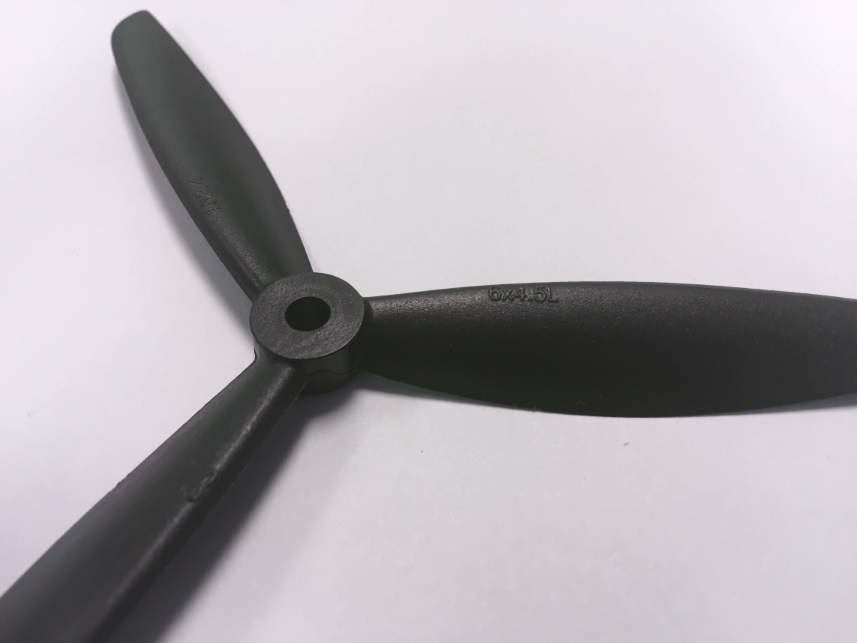
\includegraphics[width=0.8\textwidth]{figs/fixed-pitch}
\caption{Twisted, fixed pitch}
\label{fig:fixed-pitch}
\end{subfigure}
\begin{subfigure}{0.49\textwidth}
\centering
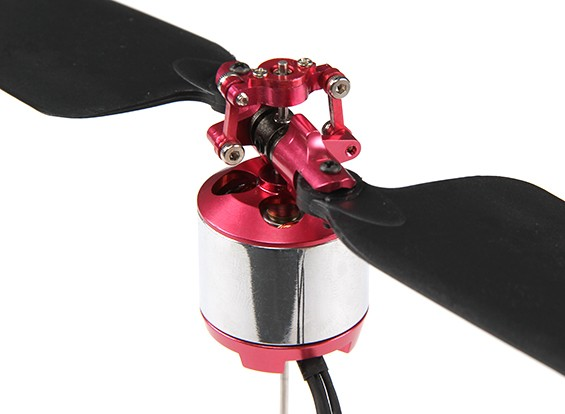
\includegraphics[width=0.8\textwidth]{figs/variable-pitch}
\caption{Variable pitch, \cite{variablepitch}}
\label{fig:variable-pitch}
\end{subfigure}
\caption{Propeller types}
\label{fig:props}
\vspace{-15pt}
\end{figure}
\par
A propeller's profile applies a perpendicular thrust force, $T$, onto the fluid in which it rotates. To build the following theoretical explanation propellers are first considered in terms of momentum theory; only perpendicular fluid flow through the propeller's plane is regarded. That fluid stream (Fig:\ref{fig:bem-flow}) has an incident upstream velocity, $v_\infty$, and a resultant slip velocity, $v_s$, downstream relative to the rotational plane.
\begin{figure}[htbp]
\centering
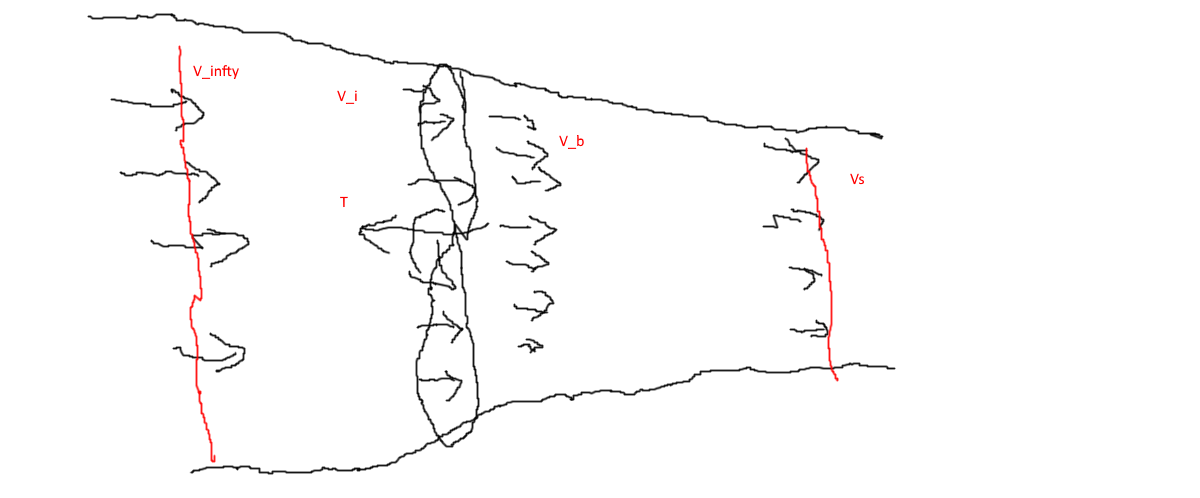
\includegraphics[width=0.6\textwidth]{figs/bem-flow}
\caption{Disc Actuator Propeller Planar Flow}
\label{fig:bem-flow}
\vspace{-15pt}
\end{figure}
\par
The change of fluid flow as a result of the propeller's rotation can be given as:
\begin{equation}
v_s = \Delta v + v_\infty
\end{equation}
Where $\Delta v$ is the net change in fluid velocity caused by the propeller blade's rotating aerofoil profile. The propeller induces a velocity directly in front of it's rotational plane, $v_i$, such that the net fluid flow into the plane is $v_b=v_i+v_\infty$. That induced inflowing fluid velocity is different to the net velocity contribution of the propeller; $v_i\not=\Delta v$. It is shown in \cite{bladesforquadrotors} that, using Bernoulli's pressure principle, the net fluid flow through the propeller's plane is:
\begin{equation}\label{eq:bernoulli}
v_b = \frac{1}{2} ( v_s - v_{\infty} ) = \frac{1}{2} \Delta v = \frac{1}{2} v_s \big|_{v_\infty=0}
\end{equation}
\newpage
Stemming from classical disc actuator (fluid \emph{momentum}) theory, the \underline{scalar} force, $T(\Omega)$, acting on the fluid is calculated as a function of mass flow rate with respect to the change in fluid velocity (pressure differential).
\begin{equation}\label{eq:prop-mass}
T=(A_b v_b)\Delta v = \rho \pi R_b^2v_b \Delta v = \rho \pi R_b^2(v_i+v_\infty)\Delta v = \frac{1}{2} \rho \pi R_b^2 \Delta v^2
\end{equation}
Where $R_b$ is the disc (propeller) radius for the fluid stream under consideration. The fluid density of that stream, $\rho$, is typically $1.225~[\text{ kg.m}^{-3}]$ at standard temperature and pressure (\emph{stp}). The desired form of thrust generated is as a function of rotational velocity $\Omega_i$, so Eq:\ref{eq:prop-mass} is not satisfactory. It can however be solved as a function of aerodynamic propulsive power expended, $\Delta P=\vec{T}\Delta v$. Rotational kinetic energy of a propeller and its transferred propulsive power is difficult to quantify, with compound parasitic losses deteriorating the efficiency of the propeller. Furthermore, the local fluid velocity through the propeller is not purely normal to the propeller plane. 
\par
The fluid flow induced by the propeller's rotation directly in front of its plane of rotation is not purely perpendicular but has axial and tangential induced velocity components, $a$ and $a'$ respectively. Those induced components for the fluid velocity can be abstracted to induction factors dependent on the incident fluid velocity to the propeller's plane of rotation:
\begin{subequations}\label{eq:induction-factors}
\vspace{-5pt}
\begin{equation}\label{eq:induction-axial}
v_i=a v_\infty~~\text{in the axial direction}
\end{equation}
\vspace{-20pt}
\begin{equation}\label{eq:induction-tangential}
v_\theta=a' \Omega_i R_b~~\text{in the tangential direction}
\end{equation}
\end{subequations}
From induction factors defined Eq:\ref{eq:induction-factors}, the velocity components can be written as functions of free upstream velocity $v_\infty$.
\begin{subequations}
\vspace{-5pt}
\begin{equation}
v_b=(1+a)v_\infty
\end{equation}
\vspace{-15pt}
\begin{equation}
v_s=(1+2a)v_\infty
\end{equation}
\end{subequations}
A consequence of the tangential fluid flow is that there exists an angular momentum flow rate across the propeller plane. This results in a torque response to the rotational motion about the propeller's axis of rotation, analogous to Eq:\ref{eq:prop-mass}.
\\
\vspace{-10pt}
\begin{equation}\label{eq:prop-moment}
\vec{Q}=\rho\pi R_b^3 (v_\theta-v_\infty) v_b 
\end{equation}
\begin{figure}[hbtp]
\vspace{-15pt}
\centering
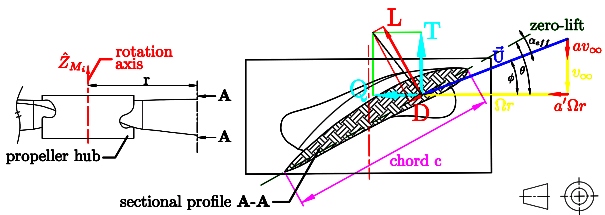
\includegraphics[width=0.9\textwidth]{figs/bem-profile}
\caption{Blade element profile at radius r}
\label{fig:bem-profile}
\end{figure}
\par
Together, Eq:\ref{eq:prop-mass} \& Eq:\ref{eq:prop-moment} make up propeller momentum theory but cannot be solved on their own. Blade-element theory analyses incremental aerofoil sections of width $dr$ of the propeller profile (Fig:\ref{fig:bem-profile}) at some radius $r$. Net local fluid velocity across a single elemental aerofoil profile $\vec{U}$ is calculated as:
\begin{equation}
\vec{U}=\sqrt{(v_\infty+v_i)^2+(v_\Omega+v_\theta)^2}
\end{equation}
Each elemental profile, of chord length $c$, has a local pitch, $\theta$, of its aerofoil zero-lift line relative to the horizontal. Local fluid velocities (again in Fig:\ref{fig:bem-profile}) encountered by the propeller make their own an angle of attack $\phi$ such that:
\begin{equation}
\phi=\theta-\alpha_{effective}
\end{equation}
That local angle of attack changes with the inflow magnitude $v_\infty$ and the induced axial velocity $v_i$. That trigonometric ratio is given as:
\begin{equation}
\phi=tan^{-1}\bigg(\frac{v_\infty+v_i}{v_\Omega+v_\theta}\bigg)=tan^{-1}\bigg(\frac{v_\infty(1+a)}{\Omega r(1+a')}\bigg)
\end{equation}
The in-plane fluid flow $\vec{U}(r,\phi)$, for an element at radius $r$ with a local angle of attack $\phi$, then contributes towards elemental lift and drag forces as a function of aerofoil's dimensionless lift, $C_L$, and drag, $C_D$, coefficients\footnote{The lift and drag coefficients are determined by the aerofoil's characteristics, but would be constant across the length of a variable pitch, non-twisted hinged propeller\ldots}.
\begin{subequations}
\begin{equation}
\Delta L=\frac{1}{2}\rho \vec{U}(r,\phi)^2 c C_L
\end{equation}
\vspace{-10pt}
\begin{equation}
\Delta D=\frac{1}{2}\rho \vec{U}(r,\phi)^2 c C_D
\end{equation}
\end{subequations}
With air density $\rho$\footnote{Typically $\rho = 1.225 kg/m^3$} and local chord length $c$. Those lift and drag forces are taken as components parallel and perpendicular to the plane of rotation. Those components are then thrust $T$ and torque $F_x$ forces (Fig:\ref{fig:bem-profile}). The in-plane force $F_x$ applies an aerodynamic torque $Q$ as the force acts at a radius $r$.
\begin{subequations}
\begin{equation}\label{eq:element-thrust}
dT=\frac{1}{2}\rho\vec{U}(r,\phi)^2c\big(C_L cos(\phi)+C_D sin(\phi)\big).dr
\end{equation}
\vspace{-5pt}
\begin{equation}\label{eq:element-drag}
dF_x=\frac{1}{2}\rho\vec{U}(r,\phi)^2c\big(C_L sin(\phi)+C_D cos(\phi)\big).dr
\end{equation}
\vspace{-5pt}
\begin{equation}\label{eq:element-torque}
\rightarrow dQ = \frac{1}{2}\rho\vec{U}(r,\phi)^2c\big(C_L sin(\phi)+C_D cos(\phi)\big)r.dr
\end{equation}
\vspace{-10pt}
\begin{equation}\label{eq:element-power}
\rightarrow dP = \Omega r dF_x .dr
\end{equation}
\end{subequations}
\par
Typically a power term, Eq:\ref{eq:element-power}, is given in lieu of torque or drag terms, Eq:\ref{eq:element-torque} or Eq:\ref{eq:element-drag}. Then calculating forces and power terms as per momentum theory for each element, in terms of axial and tangential induction factors:
\begin{subequations}\label{eq:moment-thrust-element}
\begin{equation}
dT=\rho 4 \pi r^2 v_\infty(1+a)a.dr
\end{equation}
\vspace{-10pt}
\begin{equation}
dP=\rho 4 \pi r^2 v_\infty(1+a)\Omega r (1+a').dr
\end{equation}
\end{subequations}
\par
Finally equating momentum and element terms together produces the blade-element momentum equation(s) for thrust and power produced by a propeller. Following a few assumptions, most importantly that the lift coefficient $C_L$ is a linear function of the effective angle of attack $\alpha_{eff}$. The lift curve gradient , $a_L$, for an ideally twisted blade, like the fixed pitch propellers under consideration here, is typically $2\pi$ such that $C_L=2\pi(\theta-\phi)$. And assuming that tangentially induced velocities $v_\theta$ are small (or that the tangential induction factor $a'<<1$) when compared to the propeller's speed $\Omega r$. Similarly the net inflow and axial induced velocities $v_\infty + v_i<<\Omega r$.\footnote{Small angle approximations then apply to $cos(\phi+\alpha_{eff})\approx 1$ and $sin(\phi+\alpha_{eff})\approx \phi+\alpha_{eff}$}
\newpage
\begin{subequations}
\begin{equation}\label{eq:bem-thrust}
T=\int_{r=0}^R \frac{1}{2} a_L b c \rho (\Omega r)^2 \big(\theta-\frac{v_\infty+v_i}{\Omega r}\big).dr
\end{equation}
\vspace{-3pt}
\begin{equation}\label{eq:bem-power}
P=\int_{r=0}^R \frac{1}{2}a_L b c \rho (\Omega r)^3\bigg[\big(\theta-\frac{v_\infty+v_i}{\Omega r}\big)\big(\frac{v_\infty+v_i}{\Omega r}\big) + C_d\bigg].dr
\end{equation}
\end{subequations}
With $b$ being the number of propeller blades. Generally knowing exact pitch and chord values as a function $r/R$ is difficult and calculating integrals at each process step is cumbersome. Both Eq:\ref{eq:bem-thrust} \& Eq:\ref{eq:bem-power} can be solved by equating element and momentum terms (a full expansion is given in Appendix:\ref{app:equations.bem}). Often dimensionless thrust, torque and power coefficients are defined across the entire blade's length:
\begin{subequations}\label{eq:coefficients}
\begin{equation}\label{eq:thrust-coefficient}
C_T(J)=\frac{T}{\rho \Omega^2 D^4}
\end{equation}
\vspace{-6pt}
\begin{equation}\label{eq:power-coefficient}
C_P(J)=\frac{P}{\rho \Omega^3 D^5}
\end{equation}
\end{subequations}
\par
\begin{minipage}{\textwidth}
\begin{wrapfigure}{l}{0.5\textwidth}
\vspace{-18pt}
\centering
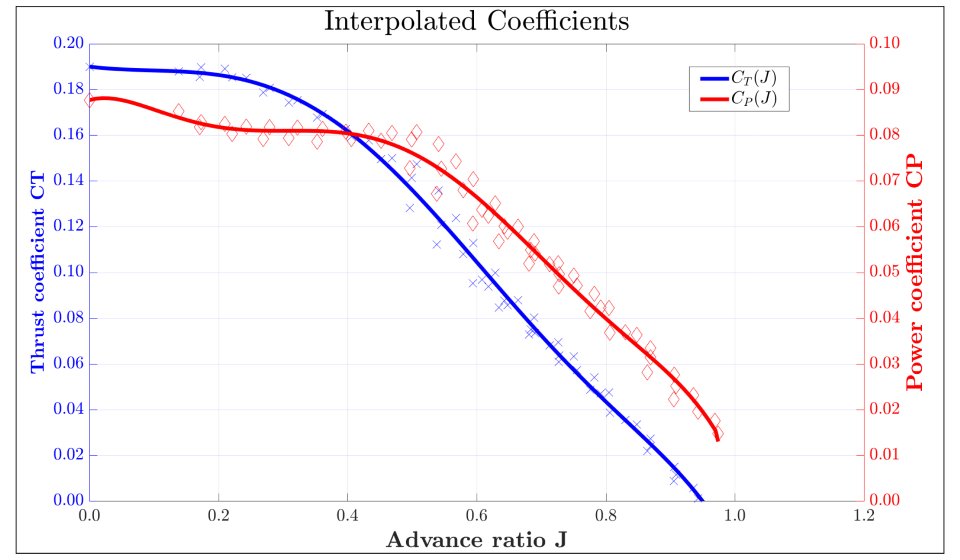
\includegraphics[width=0.5\textwidth]{graphs/coeffs-plot}
\vspace{-20pt}
\caption{Power \& thrust coefficients}
\label{fig:coeffs-plot}
\end{wrapfigure}
\par
Where $\Omega$ is the propellers rotational speed in [RPS] and $D$ is the propellers diameter in [mm]. For fixed pitch propellers the thrust and power coefficients are easily determined and remain consistent. Eq:\ref{eq:thrust-coefficient} and Eq:\ref{eq:power-coefficient} both vary due to what is defined as the \emph{advance ratio} $J$.
\begin{equation}\label{eq:advance}
J = \frac{v_\infty}{\Omega R}
\end{equation}
In most cases, the net head stream velocity $v_\infty$ is the perpendicular component (projected onto the plane's normal vector $\hat{n}$, Eq:\ref{eq:normal-fluid}) of the vehicles transnational velocity in the body frame, $\vec{v}_b\cdot\hat{n}$. For the case of a zero advance ratio, $J=0$, the conditions are regarded as static. Static thrust and power coefficients are nominal in their values. 
\end{minipage}
\par
\vspace{15pt}
Propeller databases like \cite{UIUC}\footnote{The UIUC database also includes blade profiles, pitch and chord lengths. The database is the outcome of \cite{lowreynolds}.} provide comprehensive values for a range of propeller types at different advance ratios. The introduction of those coefficients greatly simplifies the thrust estimation process. For a typical 6X4.5 inch propeller\footnote{Coefficients are linearly interpolated from similar pitched database results to match physical test values.}, the static thrust and power coefficients respectively are:
\begin{subequations}
\begin{equation}
{\color{blue}C_{T0}}=0.191
\end{equation}
\vspace{-20pt}
\begin{equation}
{\color{red}C_{P0}}=0.0877
\end{equation}
\end{subequations}
Fig:\ref{fig:coeffs-plot} shows the thrust, {\color{Blue}$C_{T}$}, and power, {\color{Red}$C_{P}$}, coefficients as a function of the advance ratio $J$. As the incident head fluid velocity, $v_\infty$, increases, the thrust coefficient decreases. So too does the power coefficient and hence the aerodynamic torque. The thrust and power coefficients can be assumed constant for low advance ratios, or in the case considered here, translational velocities.
\par
In Fig:\ref{fig:propeller-plots}, the thrust \& torque test rigs and the results of both static (thrust and torque) tests are plotted. In each test the measured values are shown ({\color{Red}$T(\Omega)$} \& {\color{Red}$Q(\Omega)$} with quadratic trend-lines) and an estimated value dependent on static coefficients ({\color{LimeGreen}$\hat{T}C_t(\Omega)$} \& {\color{LimeGreen}$\hat{Q}C_p(\Omega)$}). Using the results from the plot(s) in Fig:\ref{fig:coeffs-plot} as a lookup table and calculating the values from Eq:\ref{eq:coefficients}, induced propeller thrust and torques can be accurately modeled (\emph{quadratically}\footnote{The power term is cubic W.R.T its rotational velocity}). 
\par
Instantaneous advance ratios, or rather the propeller incident fluid flow(s), are dependent on the vehicle's net transnational and angular velocity. Such that the fluid velocity's normal component to the propeller plane is given by:
\begin{equation}\label{eq:normal-fluid}
v_\infty = (\vec{v}_b + \vec{L}_{arm}\times \vec{\omega}_b)\cdot \hat{n}
\end{equation}
Where $\vec{v}_b$ is the body's transnational velocity and $\vec{\omega}_b$ is the body's angular velocity, both transformed to the propeller's frame, $\in\mathcal{F}^{M_i}$. Furthermore $\hat{n}(\lambda_i,\alpha_i)$ is the unit vector normal to the propeller's rotational plane, dependent on the propeller's orientation relative to the body velocity. Then $J$ is calculated as in Eq:\ref{eq:advance}.
\begin{figure}[htbp]
\begin{subfigure}{0.5\textwidth}
\centering
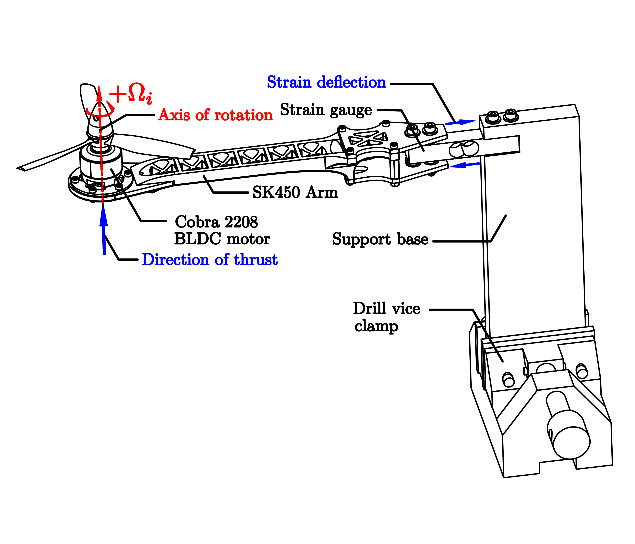
\includegraphics[width=\textwidth]{figs/thrust-rig}
\caption{Thrust test rig}
\label{fig:thrust-rig}
\end{subfigure}
\begin{subfigure}{0.5\textwidth}
\centering
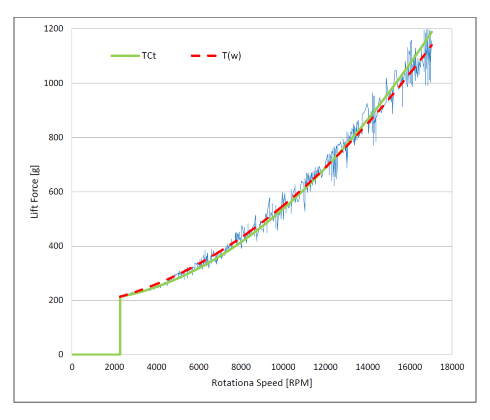
\includegraphics[width=\textwidth]{graphs/thrust-plot}
\caption{Thrust plot}
\label{fig:thrust-plot}
\end{subfigure}
\\
\begin{subfigure}{0.5\textwidth}
\centering
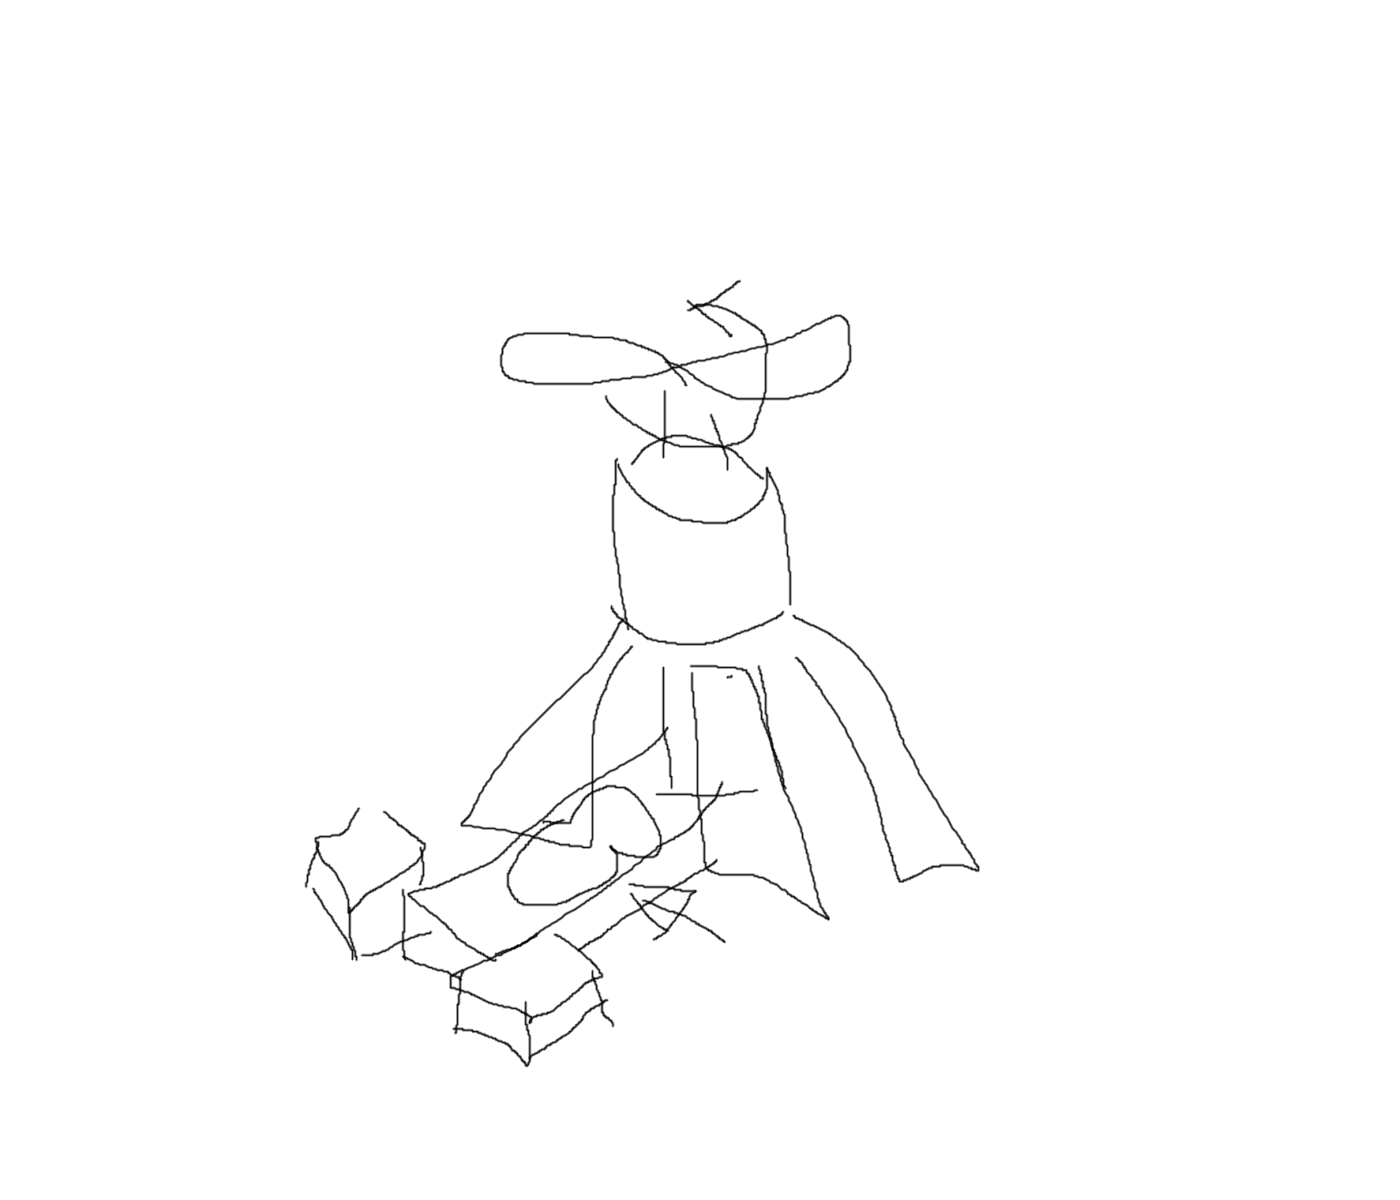
\includegraphics[width=\textwidth]{figs/torque-rig}
\caption{Torque test rig}
\label{fig:torque-rig}
\end{subfigure}
\begin{subfigure}{0.5\textwidth}
\centering
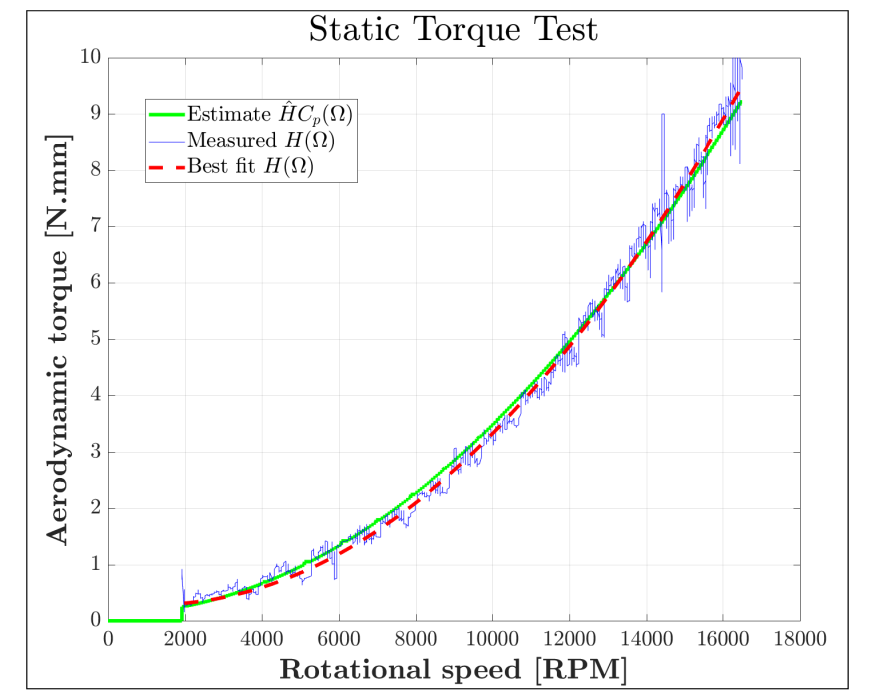
\includegraphics[width=\textwidth]{graphs/torque-plot}
\caption{Torque plot}
\label{fig:torque-plot}
\end{subfigure}
\caption{Static propeller tests}
\label{fig:propeller-plots}
\vspace{-20pt}
\end{figure}
\par
Counterclockwise and clockwise propellers and rotations were used for both thrust and torque tests. Despite the thrust and test rigs having been designed to isolate each respective response, the use of both directs allowed for opposing effects to cancel one another out. In the case of thrust tests plotted in Fig:\ref{fig:thrust-plot}; the opposing results were constructively averaged such that cross-directional torque effects on the strain gauge were cancelled out. 
\par
{\color{Gray}\emph{It's worth noting that the above static coefficients are indeed calculated from physical static tests. However advance ratio coefficient dependencies are linearly interpolated from the closest available matching data (APC Thin-Electric 8X6 propellers) cited from \cite{UIUC}}.}
\par
Conversely the recorded torque results, plotted in Fig:\ref{fig:torque-plot}, were subtractively averaged so that any erroneous perpendicular thrust deflection on the strain gauge was removed from the torque measurement. Both positive and negative rotational results for thrust and torque measurements are included in Appendix:\ref{app:thrust-torque}.
\par
{\color{Gray}\emph{Discrepancies which emerge between the model or coefficient values derived can be accounted for with lumped uncertainty disturbance term(s). Model uncertainty compensation can easily be incorporated into adaptive backstepping or $H_\infty$ control algorithms. The deviation of the modeled thrust or torques from their true values would be simple to incorporate into a plant dependent Lyapunov candidate function; Sec:\ref{subsubsec:control.attitude.nonlinear.adaptivebackstep}.}}
%====================================================
\subsection{Hinged Propeller Conning \& Flapping}
\label{subsec:dynamics.aero.flap}
%====================================================
Other non-linear effects which adversly effect a propeller's performance have all been well documented in the helicopter aerodynamic and propeller fields\cite{basichelicopter,bramwell}. Typically such affects are more pronounced when observing hinged variable pitch \footnote{Twisted, fixed pitched propellers are used on the prototype here and as such effects detailed in Sec:\ref{subsec:dynamics.aero.flap} are diminished. Moreover, low translational velocities suppress such responses but they're worth mentioning.} propellers. Conning and flapping are the two most significant aerodynamic responses produced by a propeller. Other phenomenon like cyclic vortex ring states aren't applicable here and fall outside the scope of the investigation. 
\par
\begin{figure}[htbp]
\centering
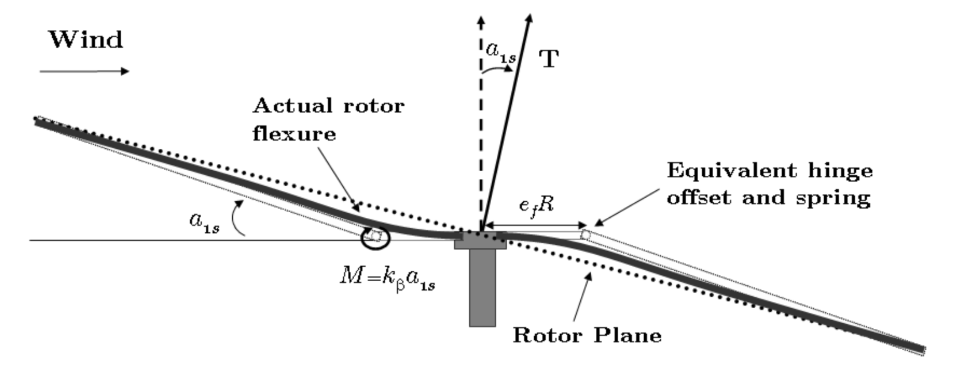
\includegraphics[width=0.95\textwidth]{figs/prop-flap}
\caption{Propeller blade flapping}
\label{fig:prop-flap}
\end{figure}
In translational flight for an unducted propeller each blade encounters varying incident fluid flow. The advancing blade, relative to the body's translational direction, encounters a greater fluid flow than the retreating blade. The result is that the effective local angle(s) of attack for the opposing advancing and retreating propeller blades aren't symmetrical. The unbalanced angles of attack produce a dissymmetry of lift across the propeller's surface.
\par
Throughout each rotation the blade is forced up and down as it cycles through varying fluid flows, applying a torque about the propeller's hub. The extent of that torque is dependent on the body's net translational velocity and the propeller material's suceptibility to deflection. The flapping pitches the effective propeller plane (\emph{tip-path plane}), and hence the thrust vector line, away from its principle axis, Fig:\ref{fig:prop-flap}\footnote{Diagram adapted from Hoffman et al.(2007)\cite{starmac}}.
\par
The overall net effect is that the propeller's thrust vector is pitched marginally away from an ideal perpendicular vector by some deflection angle. The phenomenon is diminished at low translational velocities and as such, isn't applicable to the range of flight envelopes which the prototype for this project will experience.
\par
\begin{figure}[hbtp]
\centering
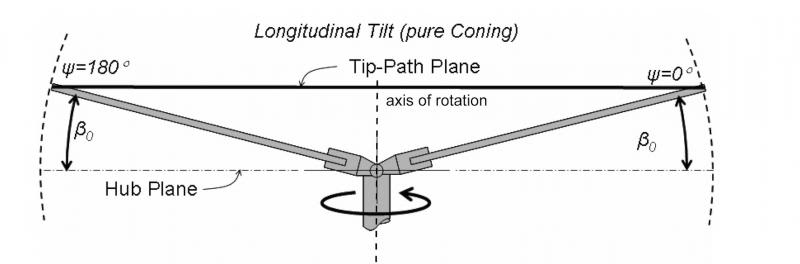
\includegraphics[width=0.95\textwidth]{figs/prop-coning}
\caption{Propeller coning}
\label{fig:prop-coning}
\end{figure}
Coning (illustrated in Fig:\ref{fig:prop-coning}) is another form of propeller deflection, which is again dependent on the blades stiffness properties, causes the propeller blades (advancing and retreating) to both deflect upward. Loading on the propeller surface and supporting a body's weight causes the upward deflection. The coning reduces the effective propeller disc's radius, adversely affecting thrust produced, Eq:\ref{eq:bem-thrust}. Increased loading accentuates the coning angle experienced by the propellers and as such alters the tip-path-plane.
\par
Both aerodynamic induced propeller deflection effects can be quantified numerically. Their derivation and resultant equations are cumbersome however. In due course their effect on the produced prototype which this project investigates isn't significant enough to produce instability if neglected. The frame could potentially be affected in more adverse ways given certain flight conditions with higher translational velocities or incident wind \& fluid flow disturbances\ldots
%====================================================
\subsection{Drag}
\label{subsec:dynamics.aero.drag}
%====================================================
For any solid body with some translational velocity motion within a fluid, there is a first order damping response opposing translational velocity. The net drag force, $\vec{D}_{net}$, although locally dependent on individual component cross-sections can be abstracted to a drag coefficient matrix representing the whole body.
\begin{equation}\label{eq:distrubance}
\vec{D}_{net}(\vec{v})=\begin{bmatrix}
A_{xx} & A_{xy} & A_{xz}\\
B_{yx} & B_{yy} & A_{yz}\\
C_{zx} & C_{zy} & C_{zz}
\end{bmatrix}
\begin{bmatrix}
u\\
v\\
w
\end{bmatrix}
~~~~\in\mathcal{F}^b
\end{equation}
\par
The drag coefficients, $A,B~\&~C$, are determined by the frames directional cross-section areas for each $\hat{X}_b,\hat{Y}_b,\hat{Z}_b$ axis. Given a well designed \& symmetrical frame, it can be assumed the off-diagonal elements aren't of consequence and as such the drag equation can be simplified to:
\begin{equation}
\vec{D}_{net}(\vec{v})\approx diag\big(A_{xx}~B_{yy}~C_{zz}\big)\vec{v}~~~~\in\mathcal{F}^b
\end{equation}
Without access to wind tunnel test facilities, the drag coefficients are difficult to empirically ascertain with a relative degree of certainty. As such the drag effects are relegated to the lumped disturbance \& uncertainty term(s) to be adpatively compensated for, Sec:\ref{subsubsec:control.attitude.nonlinear.adaptivebackstep}. Analogous drag-like opposing effects to angular rotation rates do exist but, for the intents and purposes of most practical flight envelopes, can be disregarded.
\par
In simulation; if the plant has sufficient disturbance rejection then a first order drag term in Eq:\ref{eq:distrubance} would be easily accounted for by the adaptive backstepping algorithm. It would be easy to physically test for the disturbance coefficients given further investigation on the prototype frame but, given the flight envelope for this research, is outside the scope of investigation here\ldots
%====================================================
\section{Consolidated Model}
\label{sec:dynamics.model}
%====================================================
Reiterating the different aspects detailed above and consolidating the state equations from Eq:\ref{eq:states.a}-\ref{eq:states.d}. Then lifting the attitude states to $\mathbb{R}^4$ space with the use of quaternions. Also introducing the non-linear inertial \& gyroscopic responses to induced perturbations, $\vec{\tau}_\lambda$ and $\vec{\tau}_\alpha$ from Eq:\ref{eq:torque-induced-inner} \& Eq:\ref{eq:torque-induced-middle} respectively, with non-linear inertial matrix terms $\mathbb{I}_b(u)$ from Section:\ref{sec:proto.inertia}. Finally replacing net \emph{virtual} plant inputs\footnote{Exact actuator relationships are explored in Section:\ref{sec:control.inputs}}, $\mu \vec{\tau}$ and $\mu \vec{F}$, with higher fidelity thrust models; produces the following set of state differentials used for control plant development \ldots
\\
\begin{subequations}\label{eq:quaternion-states}
\begin{equation}\label{eq:quaternion-states-velocity}
\dot{\mathcal{E}}=Q_b\otimes^*\vec{v}_b\otimes Q_b~~~~\in\mathcal{F}^I
\end{equation}
\vspace{-10pt}
\begin{equation}\label{eq:quaternion-states-acceleration}
\dot{\vec{v}}_b=m^{-1}\big(-\vec{\omega}_b\times m\vec{v}_b+Q_b\otimes m\vec{G}_I\otimes Q_b^*-\vec{D}_{net}(\vec{v}_b)+\mu\vec{F}(u)\big)~~~~\in\mathcal{F}^b
\end{equation}
\vspace{-8pt}
\begin{equation}\label{eq:quaternion-states-quaternion}
\dot{Q}_b=\frac{1}{2}Q_b\otimes \vec{\omega}_b ~~~~\in\mathcal{F}^I
\end{equation}
\vspace{-8pt}
\begin{equation}\label{eq:quaternion-states-angular}
\dot{\vec{\omega}}_b=\mathbb{I}_b(u)^{-1}\big(-\vec{\omega}_b \times \mathbb{I}_b(u)\vec{\omega}_b+\vec{\tau}_Q(u)+\vec{\tau}_g(u)+\sum \vec{Q}(\Omega,\lambda,\alpha)+\mu\vec{\tau}(u)\big)~~~~\in\mathcal{F}^b
\end{equation}
\vspace{-10pt}
\begin{equation}
u=\big[\Omega_1^+,~\lambda_1,~\alpha_1,~\ldots~\Omega_4^-,~\lambda_4,~\alpha_4 \big]~\in\mathbb{U}
\end{equation}
\end{subequations}
With net thrust and torque plant control inputs, $\mu\vec{F}$ \& $\mu\vec{\tau}$ respectively. Both are later abstracted to virtual control inputs next in Chapter:\ref{ch:control}, (\emph{individual motor number subscripts, $i\in[1:4]$, are implied}).
\begin{subequations}\label{eq:quaternion-inputs}
\begin{equation}
\mu\vec{F}(u)=\sum \vec{T}(\Omega,\lambda,\alpha)=\sum Q_{M_i}^*\otimes T(\Omega)\otimes Q_{M_i}~~~~\in\mathcal{F}^b
\end{equation}
\vspace{-6pt}
\begin{equation}
\mu\vec{\tau}(u)=\sum \vec{l}\times\vec{T}(\Omega,\lambda,\alpha)=\sum \vec{l}\times\big(Q_{M_i}^*\otimes T(\Omega)\otimes Q_{M_i}\big)~~~~\in\mathcal{F}^b
\end{equation}
\end{subequations}
The scalar thrust $T(\Omega)$ is a function of the propellers rotational velocity however $\vec{T}(\Omega,\lambda,\alpha)$ is a 3 dimensional thrust vector, redirected in the analogue of Eq:\ref{eq:motor-module-rotation.a} and transformed to the body frame $\mathcal{F}^b$. Equivalently $Q(\Omega)$\footnote{Disambiguation: $Q(\Omega)$ here is a torque, not a quaternion.} is the scalar aerodynamic torque term in $\mathcal{F}^{M_i}$ about each motor's rotor $\hat{Z}$-axis, $\vec{Q}(\Omega,\lambda,\alpha)$ is the torque vector counterpart in $\mathcal{F}^b$. Both thrust and aerodynamic propeller torque\footnote{Torque dependent on the power term calculated from Eq:\ref{eq:element-power}} terms are calculated from their respective coefficients (plotted in Fig:\ref{fig:coeffs-plot}):
\begin{subequations}
\begin{equation}\label{eq:aerodynamic-thrust}
T(\Omega)= C_T(J)\rho\Omega^2D^4
\end{equation}
\vspace{-15pt}
\begin{equation}\label{eq:aerodynamic-torque}
Q(\Omega)= C_P(J)\rho\Omega^3D^5 \frac{1}{R\Omega}
\end{equation}
\end{subequations}
Inertial torque responses from actuator input rates (\emph{in feedback\footnote{Response terms are used later as secondary actuator inputs in feedforward configuration rather than feedback terms to be compensated for.} configuration here}) from Eq:\ref{eq:torque-response};
\begin{equation}\label{eq:actuator-torque}
\tau_Q(u)=\sum_{i=1}^4 -Q_{M_i}\otimes \tau_{\lambda_i}(u)\otimes Q_{M_i}^*-Q_{M_i'}\otimes \tau_{\alpha_i}(u) \otimes Q_{M_i'}^*~~~\in\mathcal{F}^b
\end{equation}
And the variable gravitational torque arm from Eq:\ref{eq:grav-torque}, dependent on net actuator positions $u$:
\begin{equation}\label{eq:grav-torque}
\vec{\tau}_g(u)=\Delta C.G \times\vec{G}_b
\end{equation}
Finally, the body's net inertial tensor, taken from Eq:\ref{eq:body-net} is given as:
\begin{equation}
\underset{u\in\mathbb{U}}{\mathbb{I}_b(u)}=\mathbb{I}_{body}+\sum_{i=1}^{4} \mathbb{M}_{inner}+\sum_{i=1}^{4} \mathbb{M}_{middle}
\end{equation}
It is possible to bundle both attitude states (either euler angles $\vec{\eta}$ or quaternions $Q_b$) together with the linear translational position $\mathcal{E}$ into a single state vector $\mathbf{x}$. Which then has its own combined control law. This could potentially exploit the cross-product coupling terms between angular and linear displacements for control benefits.